%if printing on both sides of a page add 'twopage' to the [...] below
\documentclass[11pt,openright]{report} 
\usepackage{graphicx}
\usepackage{color}
\usepackage{tocbibind}
%\usepackage{algorithm2e} % must be included before unlv-thesis
\usepackage[linesnumbered,ruled]{algorithm2e}
\SetKwProg{Fn}{Function}{}{}
\usepackage{subcaption}
\usepackage{fancyhdr}
\usepackage{unlv-thesis}

\graphicspath{{./images/}, {./results/}}
\usepackage{hyperref}
\hypersetup{
	colorlinks=false, %set true if you want colored links
	linktoc=all,     %set to all if you want both sections and subsections linked
	linkcolor=blue,  %choose some color if you want links to stand out
}
%%%
%%% Choose either \phdthesis or \mastersthesis
\mastersthesis
%\phdthesis

%%%
%%% opens all chapters on right hand sides (needed for double sided printing)
\rightchapter
%%% add \twosided if you are printing on both sides
%\twosided
%%%
%%% Choose the spacing for the thesis: \singlespace, \oneandhalfspace or \doublespace
%\oneandhalfspace
%\singlespace
\doublespace

\makeindex

%%%
%%% The name of your thesis and your own name. Title must be in all
%%% caps and in an inverted triangle
\thesistitle{A MACHINE LEARNING APPROACH TO PREDICT FIRST-YEAR STUDENT RETENTION RATES AT UNIVERSITY OF NEVADA, LAS VEGAS}
\thesistitlelowercase{A Machine Learning Approach to Predict First-Year Student Retention Rates at University of Nevada, Las Vegas  }
\thesisauthor{Aditya Rajuladevi}

%%%
%%% Add your previous degrees here
\thesisauthorpreviousdegrees{
Bachelor Degree in Computer Engineering\\ \vspace*{-0.12in}
Jawahar Lal Nehru Technological University, Hyderabad, India\\ \vspace*{-0.12in}
2014}

%%%
%%% Month and Year to appear on the thesis
\thesismonth{May} 
\thesisyear{2018}
\copyrightyear{2018}

%%%
%%% The size of the committee: chair + other members + college rep (normally 4)
%%% use \chair{}, \memberone{}, \membertwo{}, \memberthree{}, \colleferep{}
\thesiscommitteesize{4}
%\signatures{}   % will generate 'signatures on the approval page' grad college does 
%not like this, so don't do that in their version
\chair{Fatma\ Nasoz, Ph.D.}
\memberone{Laxmi\ Gewali, Ph.D.}
\membertwo{Justin\ Zhan, Ph.D.}
\collegerep{Magdalena\ Martinez, Ph.D.}

%----------------------- Macros ----------------------------------------- 

%\newcounter{defcounter}
%\setcounter{defcounter}{1}
%\newcounter{excounter}
%\setcounter{excounter}{1}
%\newcounter{propcounter}
%\setcounter{propcounter}{1}
%\newcounter{lemmacounter}
%\setcounter{lemmacounter}{1}
%\newcounter{theoremcounter}
%\setcounter{theoremcounter}{1}                    
\newcommand{\mytheoremcounter}{section}
\newcommand{\cheapHack}{ }
\newcommand{\BAPrn}{BAP$_{\mbox{r}}$}
\newcommand{\BAPr}{BAP$_{\mbox{r}}$\ }
\newcommand{\BAPsn}{BAP$_{\mbox{s}}$}
\newcommand{\BAPs}{BAP$_{\mbox{s}}$\ }
\newcommand{\BAPsrn}{BAP$_{\mbox{sr}}$}
\newcommand{\BAPsr}{BAP$_{\mbox{sr}}$\ }
\newcommand{\BAPucn}{BAP$_{\mbox{sr}}$}
\newcommand{\BAPuc}{BAP$_{\mbox{sr}}$\ }
\newcommand{\BSPrn}{BSP$_{\mbox{r}}$}
\newcommand{\BSPr}{BSP$_{\mbox{r}}$\ }
\newcommand{\BSPsn}{BSP$_{\mbox{s}}$}
\newcommand{\BSPs}{BSP$_{\mbox{s}}$\ }
\newcommand{\BSPsrn}{BSP$_{\mbox{sr}}$}
\newcommand{\BSPsr}{BSP$_{\mbox{sr}}$\ }
\newcommand{\BSPucn}{BSP$_{\mbox{sr}}$}
\newcommand{\BSPuc}{BSP$_{\mbox{sr}}$\ }
\newcommand{\NBAPrn}{NBAP$_{\mbox{r}}$}
\newcommand{\NBAPr}{NBAP$_{\mbox{r}}$\ }
\newcommand{\NBAPsn}{NBAP$_{\mbox{s}}$}
\newcommand{\NBAPs}{NBAP$_{\mbox{s}}$\ }
\newcommand{\NBAPsrn}{NBAP$_{\mbox{sr}}$}
\newcommand{\NBAPsr}{NBAP$_{\mbox{sr}}$\ }
\newcommand{\NBAPucn}{NBAP$_{\mbox{sr}}$}
\newcommand{\NBAPuc}{NBAP$_{\mbox{sr}}$\ }
\newcommand{\fixme}[1]{$\spadesuit$\marginpar{\tiny$\spadesuit$#1}}
\newcommand{\Xhalf}{X_\frac{1}{2}}
\newcommand{\Shalf}{\cS_{\frac{n}{2},n}}
\newcommand{\chih}{\chi_n}
\newcommand{\notchih}{\overline{\chi_n}}
\newcommand{\upsh}{\upsilon_n}
\newcommand{\notupsh}{\overline{\upsilon_n}}
\newcommand{\singlespacing}{\baselineskip 1em}
\newcommand{\onehalfspacing}{\baselineskip 1.25em}
\newcommand{\doublespacing}{\baselineskip 1.75em}
\newcommand{\truedoublespacing}{\baselineskip 2em}
\newcommand{\normalspacing}{\singlespacing}
\newcommand{\Paccept}[1]{{\Pr[#1 = \mathrm{accept}]}}
\newcommand{\Maj}{\mathit{Maj}}
\newcommand{\Nand}{\uparrow}
\newcommand{\Nor}{\downarrow}
\newcommand{\myem}[1]{{\bf #1}}
\newcommand{\reccr}[1]{\overline{\nu}(#1)}
\newcommand{\regcr}[1]{\nu(#1)}
\newcommand{\LOGDCFLclass}{\mathbf{LOGDCFL}}
\newcommand{\NLclass}{\mathbf{NL}}
\newcommand{\ACclass}{\mathbf{AC}}
\newcommand{\NCclass}{\mathbf{NC}}
\newcommand{\SCclass}{\mathbf{SC}}
\newcommand{\RCclass}{\mathbf{RC}}
\newcommand{\coNLclass}{\mathbf{co\!-\!NL}}
\newcommand{\Lclass}{\mathbf{L}}
\newcommand{\Lpoly}{\mathbf{L}_{/\mathrm{poly}}}
\newcommand{\Pclass}{\mathbf{P}}
\newcommand{\BPclass}{\mathbf{P}_{BP}}
\newcommand{\BPwidth}[1]{\mathbf{P}_{BP}^{#1}}
\newcommand{\NPclass}{\mathbf{NP}}
\newcommand{\coNPclass}{\mathbf{coNP}}
\newcommand{\PPclass}{\mathbf{PP}}
\newcommand{\BPPclass}{\mathbf{BPP}}
\newcommand{\ZPPclass}{\mathbf{ZPP}}
\newcommand{\RPclass}{\mathbf{RP}}
\newcommand{\coRPclass}{\mathbf{co\!-\!RP}}
\newcommand{\SigmaP}[1]{\mathbf{\Sigma_{#1}P}}
\newcommand{\PHclass}{\mathbf{PH}}
\newcommand{\PSPACE}{\mathbf{PSPACE}}
\newcommand{\RSPACE}{\mathbf{RSPACE}}
\newcommand{\DSPACE}{\mathbf{DSPACE}}
\newcommand{\imin}{{\mathit{min}}}
\newcommand{\imax}{{\mathit{max}}}
\newcommand{\gbf}{{\mathbf{g}}}
\newcommand{\zbf}{{\mathbf{z}}}
\newcommand{\wbf}{{\mathbf{w}}}
\newcommand{\vbf}{{\mathbf{v}}}
\newcommand{\xbf}{{\mathbf{v}}}
\newcommand{\onebf}{{\mathbf{1}}}
\newcommand{\zerobf}{{\mathbf{0}}}
\newcommand{\uvec}{\vec{u}}
\newcommand{\vvec}{\vec{v}}
\newcommand{\xvec}{\vec{x}}
\newcommand{\Deltap}{\Delta^\prime}
\newcommand{\Sigmap}{{\Sigma^\prime}}
\newcommand{\alphap}{\alpha^\prime}
\newcommand{\betap}{\beta^\prime}
\newcommand{\betapp}{\beta^{\prime\prime}}
\newcommand{\gammap}{\gamma^\prime}
\newcommand{\mup}{\mu^\prime}
\newcommand{\mupp}{\mu^{\prime\prime}}
\newcommand{\nubar}{{\overline{\nu}}}
\newcommand{\nubars}{\nubar^*}
\newcommand{\nus}{\nu^*}
\newcommand{\betas}{\beta^*}
\newcommand{\deltas}{\delta^*}
\newcommand{\deltap}{\delta^\prime}
\newcommand{\deltapp}{\delta^{\prime\prime}}
\newcommand{\lambdabar}{\overline{\lambda}}
\newcommand{\lambdap}{\lambda^\prime}
\newcommand{\lambdapp}{\lambda^{\prime\prime}}
\newcommand{\pip}{\pi^\prime}
\newcommand{\pipp}{{\pi^{\prime\prime}}}
\newcommand{\Psip}{\Psi^\prime}
\newcommand{\psip}{\psi^\prime}
\newcommand{\phip}{\phi^\prime}
\newcommand{\sigmap}{\sigma^\prime}
\newcommand{\etap}{\eta^\prime}
\newcommand{\etapp}{{\eta^{\prime\prime}}}
\newcommand{\epsilonp}{{\epsilon^\prime}}
\newcommand{\epsilonpp}{\epsilon^{\prime\prime}}
\newcommand{\epsilonppp}{\epsilon^{\prime\prime\prime}}
\newcommand{\ap}{a^\prime}
\newcommand{\bp}{b^\prime}
\newcommand{\cp}{c^\prime}
\newcommand{\up}{u^\prime}
\newcommand{\fp}{f^\prime}
\newcommand{\ep}{e^\prime}
\newcommand{\gp}{g^\prime}
\newcommand{\ip}{i^\prime}
\newcommand{\jp}{j^\prime}
\newcommand{\mpr}{m^\prime}
\newcommand{\np}{n^\prime}
\newcommand{\op}{o^\prime}
\newcommand{\qp}{q^\prime}
\newcommand{\rp}{r^\prime}
\newcommand{\spr}{s^\prime}
\newcommand{\tp}{t^\prime}
\newcommand{\gpp}{g^{\prime\prime}}
\newcommand{\ipp}{i^{\prime\prime}}
\newcommand{\jpp}{j^{\prime\prime}}
\newcommand{\epp}{e^{\prime\prime}}
\newcommand{\qpp}{q^{\prime\prime}}
\newcommand{\rpp}{r^{\prime\prime}}
\newcommand{\vp}{v^\prime}
\newcommand{\ypp}{y^{\prime\prime}}
\newcommand{\xpp}{x^{\prime\prime}}
\newcommand{\zp}{z^\prime}
\newcommand{\hp}{{h^\prime}}
\newcommand{\lp}{{l^\prime}}
\newcommand{\zpp}{{z^{\prime\prime}}}
\newcommand{\kp}{{k^\prime}}
\newcommand{\Dp}{{D^\prime}}
\newcommand{\Pp}{P^\prime}
\newcommand{\Ppp}{P^{\prime\prime}}
\newcommand{\Qp}{Q^\prime}
\newcommand{\Qpp}{Q^{\prime\prime}}
\newcommand{\Spr}{S^\prime}
\newcommand{\Tp}{T^\prime}
\newcommand{\Ep}{E^\prime}
\newcommand{\Dbar}{\overline{D}}
\newcommand{\Lp}{L^\prime}
\newcommand{\Lpp}{L^{\prime\prime}}
\newcommand{\Lbar}{\overline{L}}
\newcommand{\Lhat}{\widehat{L}}
\newcommand{\Ltilde}{\tilde{L}}
\newcommand{\Lcap}{{L^\cap}}
\newcommand{\Lcup}{{L^\cup}}
\newcommand{\Lpbar}{\overline{\Lp}}
\newcommand{\Mp}{M^\prime}
\newcommand{\Mpp}{M^{\prime\prime}}
\newcommand{\Mbar}{\overline{M}}
\newcommand{\Np}{N^\prime}
\newcommand{\Npp}{N^{\prime\prime}}
\newcommand{\Rp}{R^\prime}
\newcommand{\xbar}{\bar{x}}
\newcommand{\xp}{x^\prime}
\newcommand{\yp}{y^\prime}
\newcommand{\Uhat}{\widehat{U}}
\newcommand{\Up}{U^\prime}
\newcommand{\Upp}{U^{\prime\prime}}
\newcommand{\Vp}{V^\prime}
\newcommand{\Vhat}{\widehat{V}}
\newcommand{\Vbar}{\overline{V}}
\newcommand{\Ap}{{A^\prime}}
\newcommand{\App}{{A^{\prime\prime}}}
\newcommand{\Cp}{C^\prime}
\newcommand{\Fp}{F^\prime}
\newcommand{\Gp}{G^\prime}
\newcommand{\Gtilde}{\tilde{G}}
\newcommand{\Fpp}{F^{\prime\prime}}
\newcommand{\Zf}{{\mathbb{Z}}}
\newcommand{\Qf}{{\mathbb{Q}}}
\newcommand{\Rf}{{\mathbb{R}}}
\newcommand{\Cf}{{\mathbb{C}}}
\providecommand{\mathbb}[1]{\Bbb{#1}}
\newcommand{\qacc}{q^{acc}}
\newcommand{\qrej}{q^{rej}}
\newcommand{\qnon}{q^{non}}
\newcommand{\Qadd}{Q_{add}}
\newcommand{\Qacc}{Q_{acc}}
\newcommand{\Qrej}{Q_{rej}}
\newcommand{\Qnon}{Q_{non}}
\newcommand{\Qhalt}{Q_{halt}}
\newcommand{\Qjunk}{Q_{junk}}
\newcommand{\Qaccp}{{Q_{acc}^\prime}}
\newcommand{\Qrejp}{{Q_{rej}^\prime}}
\newcommand{\Qnonp}{{Q_{non}^\prime}}
\newcommand{\Qhaltp}{{Q_{halt}^\prime}}
\newcommand{\Qjunkp}{{Q_{junk}^\prime}}
\newcommand{\Qaccpp}{{Q_{acc}^{\prime\prime}}}
\newcommand{\Qrejpp}{{Q_{rej}^{\prime\prime}}}
\newcommand{\Qnonpp}{{Q_{non}^{\prime\prime}}}
\newcommand{\Qjunkpp}{{Q_{junk}^{\prime\prime}}}
\newcommand{\Cacc}{C_{acc}}
\newcommand{\Crej}{C_{rej}}
\newcommand{\Cnon}{C_{non}}
\newcommand{\Eacc}{E_{acc}}
\newcommand{\Erej}{E_{rej}}
\newcommand{\Enon}{E_{non}}
\def\cent{{\hbox{\rm\rlap/c}}}
\newcommand{\centp}{{\cent}^\prime}
\newcommand{\Bra}[1]{{\langle{#1}|}}
\newcommand{\Ket}[1]{{|{#1}\rangle}}
\newcommand{\BraKet}[2]{{\langle{#1}|{#2}\rangle}}
\newcommand{\iprod}[2]{{\langle{#1},{#2}\rangle}}
\newtheorem{theorem}{{\bf Theorem}}[\mytheoremcounter]
\newtheorem{lemma}[theorem]{{\bf Lemma}}
\newtheorem{aside}[theorem]{{\bf Aside}}
%\newtheorem{claim}[theorem]{{\bf Claim}}
\newtheorem{example}[theorem]{{\bf Example}}
\newtheorem{question}[theorem]{{\bf Question}}
\newtheorem{answer}[theorem]{{\bf Answer}}
\newtheorem{conjecture}[theorem]{{\bf Conjecture}}
\newtheorem{proposition}[theorem]{{\bf Proposition}}
\newtheorem{property}[theorem]{{\bf Property}}
\newtheorem{corollary}[theorem]{{\bf Corollary}}
\newtheorem{observation}[theorem]{{\bf Observation}}
%\newtheorem{fact}[theorem]{{\bf Fact}}
\newtheorem{definition}[theorem]{{\bf Definition}}
\newtheorem{remark}[theorem]{{\bf Remark}}
\newtheorem{thoughts}[theorem]{{\bf Thoughts}}
\newenvironment{proof}{ \begin{trivlist} 
                        \item \vspace{-\topsep} \noindent{\bf Proof:}\ }
                      {\rule{5pt}{5pt}\end{trivlist}}
\newcommand{\Subcase}[2]{\noindent{\bf Subcase #1:}#2}
\newcommand{\Half}{\frac{1}{2}}
\newcommand{\RtHalf}{\frac{1}{\sqrt{2}}}
\newcommand{\cA}{{\mathcal{A}}}
\newcommand{\cC}{{\mathcal{C}}}
\newcommand{\cE}{{\mathcal{E}}}
\newcommand{\cF}{{\mathcal{F}}}
\newcommand{\cH}{{\mathcal{H}}}
\newcommand{\cI}{{\mathcal{I}}}
\newcommand{\cK}{{\mathcal{K}}}
\newcommand{\cL}{{\mathcal{L}}}
\newcommand{\cM}{{\mathcal{M}}}
\newcommand{\cO}{{\mathcal{O}}}
\newcommand{\cP}{{\mathcal{P}}}
\newcommand{\cR}{{\mathcal{R}}}
\newcommand{\cS}{{\mathcal{S}}}
\newcommand{\cU}{{\mathcal{U}}}
\newcommand{\Span}{{\mathit{Span}}}
\newcommand{\Ch}[2]{{#1 \choose #2}}
\newcommand{\Ul}[1]{{\underline{#1}}}
\newcommand{\Floor}[1]{{\lfloor #1 \rfloor}}
\newcommand{\ignore}[1]{}
\newcommand{\noignore}[1]{#1}

\newcommand{\RMO}{\mathbf{RMO}}
\newcommand{\UMO}{\mathbf{UMO}}
\newcommand{\RMOe}{\mathbf{RMO}_\epsilon}
\newcommand{\RMM}{\mathbf{RMM}}
\newcommand{\UMM}{\mathbf{UMM}}
\newcommand{\RMMe}{\mathbf{RMM}_\epsilon}

\newcommand{\MOQFA}{\mathbf{MOQFA}}
\newcommand{\MOQFAe}{\mathbf{MOQFA}_\epsilon}
\newcommand{\MMQFA}{\mathbf{MMQFA}}
\newcommand{\MMQFAe}{\mathbf{MMQFA}_\epsilon}
\newcommand{\GQFA}{\mathbf{GQFA}}
\newcommand{\GQFAe}{\mathbf{GQFA}_\epsilon}

\newcommand{\REG}{\mathbf{REG}}
\newcommand{\PFA}{\mathbf{PFA}}
\newcommand{\PFAe}{\mathbf{PFA}_\epsilon}
\newcommand{\GFA}{\mathbf{GFA}}

% Code environment
\newcommand{\Foreach}[2]{\\{\bf\tt{for\ each}} $#1$ {\bf\tt{do}}\+ #2
\- \\ {\bf\tt{rof}}}
\newcommand{\Forloop}[2]{\\{\bf\tt{for}} $#1$ {\bf\tt{do}}\+ #2
\- \\ {\bf\tt{rof}}}
\newcommand{\Ifthen}[2]{\\{\bf\tt{if}} $#1$ {\bf\tt{then}}\+ #2
\- \\ {\bf\tt{fi}}}
\newcommand{\Ifelse}[3]{\\{\bf\tt{if}} $#1$ {\bf\tt{then}}\+ #2
\- \\ {\bf\tt{else}}\+ #3 \- \\ {\bf\tt{fi}}}
\newcommand{\Stmt}[1]{\\$#1$;}
\newcommand{\StartStmt}[1]{\+\kill$#1$;}
\newenvironment{pseudocode}{\begin{tabbing} 
\ \ \ \ \=\ \ \ \ \=\ \ \ \ \=\ \ \ \ \=\ \ \ \ \=\ \ \ \ \=\ \ \ \ \=\
\ \ \ \= } {\end{tabbing}}

% Moving proofs around
% #1 = proof \name   #2 = appendix ref    #3 = proof
\providecommand{\SaveProof}[3]{#3}
% #1 = proof \name   #2 = appendix ref    #3 = proof    #4 = sketch
\providecommand{\SketchProof}[4]{#3}
% #1 = proof \name   #2 = appendix label  #3 = title
\providecommand{\AppendixProof}[3]{}

\newcommand{\MoveProofsToAppendix}{\include{movemacs}}

% Short equation separator
\newcommand{\ShortSep}{\\ & &}
\newcommand{\LongSep}{}
\providecommand{\DefSep}{\LongSep}
\newcommand{\UseShortSep}{\renewcommand{\DefSep}{\ShortSep}}


% select abstract mechanism
\newcommand{\UseAbstract}[2]{#1}
\newcommand{\UseOtherAbstract}{\include{absselect}}

% EVIL stuff to make it fit for 10 page limit (two lines per page extra)
\newcommand{\StretchPage}{ \addtolength{\textheight}{0.05\textheight}
                           \addtolength{\topmargin}{-0.03\textheight}
                         }

% figure macro

\newcommand{\DoFigure}[4]{
                          \begin{figure}[ht]
\setlength{\topsep}{-10pt}
\setlength{\parsep}{0pt}
\setlength{\partopsep}{0pt}
\setlength{\parskip}{0pt}
                            \begin{center}
                              \ \includegraphics[scale=#2]{#1}\ 
                            \end{center}
                            \caption{#3\label{#4}}
                          \end{figure}
                         }

\newcommand{\DoBiFigure}[5]{
                          \begin{figure}[ht]
\setlength{\topsep}{-10pt}
\setlength{\parsep}{0pt}
\setlength{\partopsep}{0pt}
\setlength{\parskip}{0pt}
                            \begin{center}
                              \mbox{\ \includegraphics[scale=#3]{#1}\ 
                                    \hspace{1.0in}
                                    \ \includegraphics[scale=#3]{#2}\ }
                            \end{center}
                            \caption{#4\label{#5}}
                          \end{figure}
                         }

\newcommand{\DoDiFigure}[8]{ 
                          \begin{figure}[ht]
\setlength{\topsep}{-10pt}
\setlength{\parsep}{0pt}
\setlength{\partopsep}{0pt}
\setlength{\parskip}{0pt}
                            \begin{center}
                              \begin{minipage}[b]{0.35\linewidth}
                                \begin{center}
                                  \includegraphics[scale=#2]{#1}
                                \end{center}
                                \caption{#3\label{#4}}
                              \end{minipage}
                              \hspace{1.0in}
                              \begin{minipage}[b]{0.35\linewidth}
                                \begin{center}
                                  \includegraphics[scale=#6]{#5}
                                \end{center}
                                \caption{#7\label{#8}}
                              \end{minipage}
                            \end{center}
                          \end{figure}
                         }

\newcommand{\DoTable}[3]{
                          \begin{table}[ht]
                            \begin{center}
                              #1
                            \end{center}
                            \caption{#2\label{#3}}
                          \end{table}
                         }


\newcommand{\pseudosection}[1]{\vspace{\baselineskip}
\noindent{\sffamily\bfseries #1}\vspace{0.5\baselineskip}}
\newcommand{\mycaption}[3]{
 \begin{center}
   \parbox{0.90\columnwidth}{\caption[#1]{
     \setlength{\baselineskip}{1.3\baselineskip}
     #2}\label{#3}}
 \end{center}}



%---------------------- Thesis starts here ------------------------------

% The organization should be as follows, as per our online guidelines:
% page (not numbered): title page
% page (not numbered): copyright statement (this page is optional)
% page ii: approval page, but do not inlcude it until the grad college says ok.
% page iii:  abstract
% acknowledgments
% preface
% table of contents
% list of tables 
% list of figures
% page 1 -> ???: main body of text
% exhibits (what ever that is)
% appendices
% bibliography,
% author's CV. 

% everything after main body should have regular page numbers, 
% everything before should have roman numeral in small letters.
\begin{document}
\thesistitlepage
\copyrightpage

\newpage
%% here goes the approval page - uncomment the following line when you 
%% get an ok from the graduate college:
%%
%% \approvalpage for the page that people need to sign
%%
%% \electronicapprovalpage for the page that needs to be used when submitting the PDF

%\approvalpage
\electronicapprovalpage


\begin{thesisabstract}
First-Year student retention rates refer to the percentage of first-year students who return to the same institution for their sophomore year. The national average in the institutions at the U.S for the year 2016 is at around 77 \% which indicates that most of the universities are performing poorly in terms of retaining the first-year students. First-year retention rates act as an important indicator of the student satisfaction as well as the performance of the university. Moreover, universities with low retention rates may face a decline in the admissions of talented students with a notable loss of tuition fees and contributions from alumni. Hence it became important for universities to formulate strategies to identify students at risk and take necessary measures to retain them. Many universities have tried to develop successful intervention programs to help students increase their performance. However, identifying and prioritizing students who need early interventions still remains to be very challenging.  

The retention rate at the University of Nevada, Las Vegas (UNLV) is close to 74\% which indicate the need for specific intervention programme's to retain the students at risk of dropping out after their first year. In this thesis, we propose the use of predictive modeling methods to identify students who are at risk of dropping out after their first year at an early stage to whom the instructors can offer help. We apply several important classification algorithms from machine learning such as Logistic Regression, Decision trees, and Random forest classifier and evaluate them using metrics useful to the educators at UNLV. We use feature selection methods to identify important variables used in each model to increase the generalization and accuracy of the predictions. We propose to design effective metrics to evaluate the model's performance to help match at-risk students with appropriate supports. The main focus of this research is on students at risk of not being retained at the end of the first year, but it also lays a foundation for future work on other adverse academic outcomes. 
\end{thesisabstract}


%%% if you have a preface it should go here before the acknowledgement


%%%
%%% Here goes the acknowledgements if you have any - if none then delete or
%%% comment out completely
\begin{thesisacknowledgments}
I would like to express my sincere gratitude to my advisor, Dr. Fatma Nasoz, for her motivation, guidance, and support throughout the research. She continuously steered me in the right direction in this research as well as my Master's program.

I would also like to extend my thanks to Dr. Laxmi Gewali, Dr. Justin Zhan, and Dr. Magdalena Martinez for their support and for being a part of my thesis committee. I am really grateful for all the support from Dr. Ajoy K Datta who was always available to me whenever I needed his guidance.

I am gratefully indebted to Kivanc Oner, Carrie Trentham and Becky Lorig from the Enterprises Application Services department at UNLV for their continuous support and valuable comments on this thesis. They answered my many questions about student enrollments and retention problems at UNLV and played a major role in helping me find the student data I was looking for from the UNLV data warehouse.

My deep sense of gratitude to my parents Venkat Rao Rajuladevi, Mallika Rajuladevi and my sister Arthi Rajuladevi who are my moral strength and motivation. I would like to thank Sai Phani Krishna Parsa for his constant support and guidance throughout my Master's program.

Finally, I would like to thank all my friends, seniors and juniors who made my time here at UNLV very memorable. 
\end{thesisacknowledgments}

%%%
%%% Magic. If you remove this you will not get page numbers on 
%%% any 2nd, 3rd or so on page of any of the tableofcontents
%%% or listofXXXX
%%%
\fancypagestyle{plain}{%
  \fancyhf{}
\renewcommand{\headrulewidth}{0.0pt}
\renewcommand{\footrulewidth}{0.0pt}
  \fancyfoot[C]{\thepage}
}
\pagestyle{plain}

%%%
%%% If you don't want list of figure and list of tables then just put a % 
%%% in front of the two lines here:
\tableofcontents
\clearpage
\listoftables
\clearpage
\listoffigures
\clearpage
% if you want a list of algorithms, make sure to use the Makefile-loa instead of Makefile.
\listofalgorithmes
\clearpage

%%%
%%% This is the start of the first 
\chapter{Introduction}\label{chapter:introduction} 

The first-year or freshmen retention rate refers to the number of freshmen in a college or university who return for their sophomore year. Many universities are facing huge problems with low or decreasing first-year student retention rates. Low retention rates are a bad indicator of the university's performance and can damage the reputation of the institution in the eyes of students and parents. The reasons behind student dropout after the first year in universities can range from high expectations of the college programs, transition into an interdisciplinary curriculum, economic problems, inability to mix well with other students or struggling due to unfulfilled prerequisite requirements \cite{lau2003institutional}. Many researchers have formulated solutions such as building learning communities, providing additional resources \cite{tinto1999taking}, highlighting student participation in campus life and providing academic support \cite{lau2003institutional}. Also, few studies have indicated that the risk of dropping out decreases with an increase in academic performance \cite{Murtaugh}. Thus, one way to increase retention is to increase academic success. In recent years, many universities have invested significantly in development and implementation of intervention programs to help at-risk students and support them individually to improve their academic performance. 

The success of such intervention programs depends on the university's ability to accurately identify students who need help. In a traditional approach, many universities have used academic performance indicators such as GPA's, absence rates, previous grades, SAT or ACT scores from enrollment data to generate rules that can be used to identify students at risk \cite{bingham2016}. Although such rule-based systems served as good indicators of identifying at-risk students for some years, they had some downsides such as fewer accuracies, static,  expensive to generate and maintain and most importantly they lacked a validation mechanism to verify the predictions. Alternatively, recent research has indicated the potential value of machine learning algorithms such as Logistic Regression, Random Forest Classifiers, Decision Trees, Support Vector Machines (SVM) and Neural networks for the problem \cite{plagge2013using,lakkaraju2015machine,marbouti2016models}. These algorithms when trained using traditional academic data can identify at-risk students more accurately. The performance of these algorithms can be evaluated using various metrics such as Precision, Recall, and Area Under Curve (AUC) thus giving us a good indicator to validate the results. However, the application of such predictive methods to identify at-risk students is still at its early stages, owing to the implementation complexity and the availability of data. Currently, many universities have defined rules in the collection of data to use for such a research.

Over the recent years, the retention rates at UNLV have displayed a highly varying pattern. It dropped from 77\% in 2012 to 74\% in 2014 and then increased to 77\% in 2015, which later on fell to 74\% in 2016 Figure \ref{fig:unlv_retention_trend}. Such an unstable pattern of freshmen retention rates has drawn a lot of attention by the educators and administration at UNLV. Hence, a predictive approach to identifying at-risk students and supporting them with additional resources would be quite beneficial to increase the retention rates at UNLV. 

\begin{figure}
	\centering
	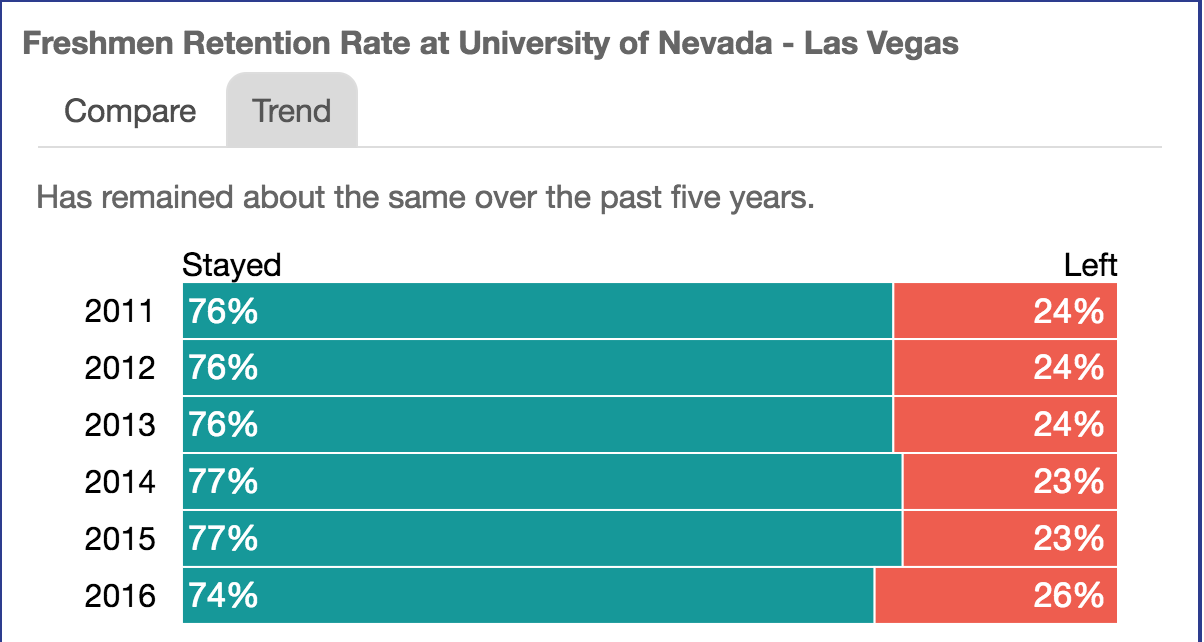
\includegraphics[scale=0.7]{unlv-retentiontrend}
	\caption{Freshmen Retention Rates at UNLV}
	\label{fig:unlv_retention_trend}
\end{figure}

\section{Objective}\label{section:objective}
The objective of this thesis is to create predictive models that can be used to identify at-risk students. In this thesis, important machine learning algorithms such as Logistic Regression, Decision trees, Random Tree Classifiers and SVM's will be trained on real-time student data obtained from UNLV's enrollment census. The trained models will then be used to predict at-risk students from a test dataset which the model has not seen earlier. The models are evaluated and compared using metrics such as precision, recall, and area under the curve to determine which model provides the best results. The results of the analysis such as the evaluation metrics will be converted to risk scores which can be easily understood by the educators and administrators at UNLV. Another contribution of this thesis is to rank students based on risk scores which will be very helpful in an efficient allocation of resources as part of the intervention programs.

\section{Outline}\label{section:outline}

In Chapter \ref{chapter:introduction}, the brief topic of First-Year student retention rates, its importance to universities and the proposed approach to increase the retention rates at UNLV was described.\newline

\noindent In Chapter \ref{chapter:background}, we will discuss the existing research on improving first-year retention rates and the background information required to understand the proposed predictive approach using machine learning. It will also cover the most important and popular algorithms of machine learning.
\newline

\noindent In Chapter \ref{chapter:proposed_system}, we will propose two methods to find the high utility itemsets. One method will be based on the pruning strategies approach which is suitable for the smaller datasets while another method will be based on the distributed computing approach for the very large datasets. The detailed description will be provided along with the examples of these methods.
\newline

\noindent In Chapter \ref{chapter:experiment_results}, we will present the experimental results showing the difference between our methods and the state-of-the-art algorithms based on the time, accuracy and efficiency. The characteristics of datasets used for these methods will also be described.
\newline

\noindent In Chapter \ref{chapter:conclusion}, we will summarize the proposed methods and their results along with the possible extension of this thesis.

\chapter{Background and Preliminaries} \label{chapter:background}
\section{Related Work}\label{section:relatedwork}

The prediction of first-year student retention rates and identification of students at risk of not being retained has been a well-researched problem in the area of higher education sector for decades. Early studies involved learning the important factors that lead to student dropout by developing a theoretical model. Tinto is one of the major and earliest researchers in this area. Tinto's student engagement model \cite{tinto1999taking} has served as the basis for a large number of theoretical studies \cite{braxton2002introduction}. Similar research was carried out by Ernest Pascarella, Patrick Terenzini, and Alexander Astin, which focused more on the external factors such as the institution's administration and its policies when determining the reasons for student retention \cite{astin2012assessment}. Tinto in his 2006 study \cite{tinto2006} has stated that there has been a huge increase in the number of businesses and organizations to analyze and help institutions with the student retention problem. Later, in the same study, he revealed that there was only little change in the retention rates even with some huge businesses helping the universities. He also described the importance of external factors such as student-faculty relationships, extracurricular program, and orientation programs for first years. Moreover, he incorporated the role of academic factors into his model to make it more suitable to the college structure \cite{tinto2006}. Astin in his Input-Environment model \cite{astin2012assessment}, suggests that researchers should consider pre-college factors such as gender, race/ethnicity, family background, high school GPA  as important for student retention.

In addition to understanding the factors responsible for student dropout, the researchers were interested in identifying students at risk of not being retained in order to intervene and prevent them from dropping out. Early research included usage of statistical and analytical methods such as logistic regression and discriminant analysis for predicting student retention rates\cite{lakkaraju2015machine,marbouti2016models,adejo2017}. The results from these models showed that the learning algorithms were in fact better than many existing rule based models in learning patterns from the existing student data. Educational data mining has emerged into an important field of research in studying student retention, because of its high accuracy and robustness in working with missing data been\cite{alkhasawneh2014developing}. In another study, Jay Bainbridge, James Melitski, Anne Zahradnik, Eitel J. M. Lauría, Sandeep Jayaprakash and Josh Baron used fall 2010 undergraduate students data from four different sources and applied classifiers such as logistic regression, support vector machines and c4.5 decision trees for prediction and comparison purposes\cite{bainbridge2015}. The results showed that logistic regression and SVM trees provided higher classification accuracies compared to the decision trees to predict students at risk. 

Serge Herzog a researcher from University of Nevada, Reno(UNR) campus has done some extensive research on student retention and graduate prediction. He used Decision trees and Neural networks to predict student retention of data from UNR\cite{herzog2006estimating}. FarshidMarbouti, Heidi A.Diefes-Dux, KrishnaMadhavan \cite{marbouti2016models} have compared seven different prediction models for identifying at-risk students using in-semester performance factors (i.e., grades) and based on standards-based grading.Another similar research focused on the problem of imbalanced output class distribution in the field of student retention in which the researchers tested three balancing techniques such as over-sampling, under-sampling and synthetic minority over-sampling (SMOTE) along with machine learning algorithms.

Although predictive analysis using machine learning models have proved to be very effective in identifying at-risk students, they were still not efficient and useful to educators who wanted to develop academic support programs and resources to support the identified students. The primary reason being the lack of understanding of the metrics from the predictive models by the educators. A few researchers analyzed this issue at the high school level and came up with a framework to convert model accuracies to risk scores that could be used by the educators in the efficient allocation of the resources \cite{lakkaraju2015machine}. Though the above-mentioned framework was giving good results, it was restricted to school level data and thus cannot yield accurate results in the university level as both are very different environments with different set of factors. Hence, in this thesis we try to include such an analysis into college level studies of UNLV and compare our results to the existing approaches.


\section{Preliminaries}\label{section:preliminaries}
\subsection{High Utility Itemset Mining}
Let us suppose the transactional database with set of transactions $D = {T_1, T_2, ...., T_n}$ which has the finite set of m unique items $I = {i_1, i_2, ...., i_m}$. Each transaction in database, $T_q \in D$ where $1 \leq q \leq n$ has a unique identifier, called its Transaction ID (TID). Each item $i_j$ is associated with quantity, which is internal utility, and with its associated profit value, which is external utility. Internal utility is denoted by $q(i_j, T_q)$ and external utility by $pft(i_j)$. A set of k unique items $X = {i_1, i_2, ...., i_k}$ where $X \subseteq I$ is said to be a k-itemset, where k is the length of an itemset and an itemset X is in transaction $T_q$ if $X \subseteq T_q$ and a minimum threshold ratio $\delta$ is defined.

\begin{table}[!t]
	\renewcommand{\arraystretch}{1.3}
	\caption{A Transactional Database D}
	\label{table:quantitative_db}
	\centering
	\begin{tabular}{|c||c||c|}
		\hline
		\bfseries TID & \bfseries Transaction (item:quantity) & \bfseries TU\\
		\hline\hline
		$T_1$ & A:3, B:2, D:2 & 17\\ \hline
		$T_2$ & A:4, C:1, D:3, E:2 & 15\\ \hline
		$T_3$ & A:2, B:1, E:3, F:5, G:2 & 22\\ \hline
		$T_4$ & B:2, C:1, E:3 & 16\\ \hline
		$T_5$ & B:1, C:1, E:1, F:1 & 11\\ \hline
	\end{tabular}
	
	\bigskip
	
	\renewcommand{\arraystretch}{1.3}
	\caption{A Profit Table}
	\label{table:profit_table}
	\centering
	\begin{tabular}{|c||c|}
		\hline
		\bfseries Item & \bfseries Profit Value\\
		\hline\hline
		$A$ & 1\\ \hline
		$B$ & 5 \\ \hline
		$C$ & 3\\ \hline
		$D$ & 2\\ \hline
		$E$ & 1\\ \hline
		$F$ & 2\\ \hline
		$G$ & 1\\ \hline
	\end{tabular}
\end{table}

An illustrative example is shown in Table \ref{table:quantitative_db} which represents the quantitative (transactional) database. There are five transactions with seven distinct items in the quantitative database. Table \ref{table:profit_table} represents the profit table which contains profit value for each item. The user specified threshold ratio $\delta$ is taken as $30.86\%$ which will be threshold value of $25 (TU \times \delta)$.


\begin{definition}
	The utility of an item $i_j$ denoted by $u(i_j, T_q)$ in a transaction $T_q$ is defined as,
	\begin{equation}
	u(i_j, T_q) = q(i_j, T_q) \times pft(i_j)    \label{eq:utilItemTran}
	\end{equation}
\end{definition}
The utility of items $A$, $B$ and $D$ in transaction $T_1$ are calculated using the Equation \ref{eq:utilItemTran} as,\\
\indent $u(A,T_1) = q(A,T_1) \times pft(A) = 3 \times 1 = 3$\\
\indent $u(B,T_1) = q(B,T_1) \times pft(B) = 2 \times 5 = 10$\\
\indent $u(D,T_1) = q(D,T_1) \times pft(D) = 2 \times 2 = 4$

\begin{definition}
	The utility of an itemset X denoted by $u(X, T_q)$ in a transaction $T_q$ is defined as,
	\begin{equation}
	u(X, T_q) = \sum_{i_j \subseteq X \cap X \subseteq T_q} u(i_j, T_q) \label{eq:utilItemsetTran}
	\end{equation}
\end{definition}
 The utility of itemsets in transaction $T_1$ is calculated from Equation \ref{eq:utilItemsetTran} as,\\ 
\indent $u(AB,T_1) = u(A,T_1) + u(B,T_1) = 3 + 10 = 13$ \\
\indent $u(ABD,T_1) = u(A,T_1) + u(B,T_1) + u(D,T_1) = 3 + 10 + 4= 17$ 

\begin{definition}
	The utility of an itemset X denoted by $u(X)$ in database $D$ is defined as,
	\begin{equation}
	u(X) = \sum_{X \subseteq T_q \cap T_q \in D} u(X, T_q) \label{eq:utilityItemsetDB}
	\end{equation}
\end{definition}
The utility of itemsets C and D in database D is calculated from Equation \ref{eq:utilityItemsetDB} as, \\
\indent $u(AB) = u(AB,T_1) + u(AB,T_3) = 13 + 7 = 20$.

\begin{definition}
	The transaction utility of a transaction $T_q$ denoted by $TU(T_q)$ is defined as,
	\begin{equation}
	TU(T_q) = \sum_{X \subseteq T_q} u(X, T_q) \label{eq:tranUtil}
	\end{equation}
\end{definition}
The transaction utility of a transaction $T_1$ is calculated from Equation \ref{eq:tranUtil} as,\\
\indent$TU(T_1) = u(A,T_1) + u(B,T_1) + u(D,T_1) = 3 + 10 + 4 = 17$.\\
Similarly, the total utility for other transactions are $T_2 = 15, T_3 = 22, T_4 = 16$ and $T_5 = 11$ as shown in Table \ref{table:quantitative_db}.

\begin{definition}
	The total utility denoted by $TU$ in database $D$ is defined as,
	\begin{equation}
	TU = \sum_{T_q \in D} TU(T_q) \label{eq:totalUtil}
	\end{equation}
\end{definition}
 The total utility is calculated from Equation \ref{eq:totalUtil} as,\\
 \indent $TU = 17 + 15 + 22 + 16 + 11 = 81$.

\begin{definition}
	The transaction weighted utility of an itemset X denoted by $TWU(X)$ in database $D$ is defined as,
	\begin{equation}
	TWU(X) = \sum_{X \subseteq T_q \in D} TU(T_q) \label{eq:twuItemset}
	\end{equation}
\end{definition}
 The transaction weighted utility for an itemset \{A,B\} is calculated from Equation \ref{eq:twuItemset} as,\\
 \indent$TWU(AB) = TU(T_1) + TU(T_3) = 17 + 22 = 39$.

\begin{definition}
	An itemset X in a database D is a high transaction weighted utility itemset (HTWUI) if its TWU is greater than or equal to the minimum threshold, where minimum threshold is $TU$ multiplied by user specified threshold ratio $\delta$ as,
	\begin{equation}
	HTWUI \gets \{X|TWU(X) \ge TU \times \delta \} \label{eq:htwui}
	\end{equation}
\end{definition}
Since an itemset $\{A,B\}$ has $TWU(AB) \ge TU \times \delta (81 \times 30.86 = 25)$, it is therefore a high transaction weighted utility itemset. 


\begin{definition}
	An itemset X in a database D is a high utility itemset ($HUI$) if its utility is greater than or equal to the minimum threshold, where minimum threshold is $TU$ multiplied by user specified threshold ratio $\delta$ as,
	\begin{equation}
	HUI \gets \{X|u(X) \ge TU \times \delta \} \label{eq:hui}
	\end{equation}
\end{definition}
An itemset $\{A,B\}$ has $u(AB) \le TU \times \delta$, it is not a high utility itemset ($HUI$). Similarly, an itemset $\{B,E\}$ has $u(BE) \ge TU \times \delta$, it is a HUI.

\begin{definition}
	\label{def:total_ordering}
	The total ordering denoted by $\rightarrow$ is the ordering of items in the increasing order of transaction weighted utility in the transaction. 	
\end{definition}
The transaction weighted utility for each item is as shown in the Table \ref{table:twu_items}. The increasing order of items in terms of TWU is: $G, D, F, C, A, E, B$ ($G \rightarrow D \rightarrow F \rightarrow C \rightarrow A \rightarrow E \rightarrow B$).

\begin{table}
	\renewcommand{\arraystretch}{1.3}
	\caption{Transaction Weighted Utility of 1-TWU Items}
	\label{table:twu_items}
	\centering
	\begin{tabular}{|c||c|c|c|c|c|c|c|}
		\hline
		\bfseries Itemset & \bfseries \{A\} & \bfseries \{B\} & \bfseries \{C\} & \bfseries \{D\} & \bfseries \{E\} & \bfseries \{F\} & \bfseries \{G\}\\
		\hline
		$TWU$ & 54 & 66 & 42 & 32 & 64 & 33 & 22\\ \hline
	\end{tabular}
\end{table}

\begin{definition}
	The revised transaction ($RT$) is said to be a transaction in which all the items which have $TWU \le TU \times \delta$ are removed and the items remaining are sorted in increasing order of $TWU$. The items that are removed from the transactions are said to be unpromising items.
\end{definition}
From the given illustrative example in Table \ref{table:quantitative_db} and Table \ref{table:profit_table}, the revised transactional database after removing the unpromising items and the items arranged in increasing order of TWU are as shown in Table \ref{table:revisedDatabase}.

\begin{table}
	\renewcommand{\arraystretch}{1.3}
	\caption{Revised Transactional Database}
	\label{table:revisedDatabase}
	\centering
	\begin{tabular}{|c||c||c|}
		\hline
		\bfseries TID & \bfseries Transaction (item:utility)\\
		\hline\hline
		$T_1$ & D:4, A:3, B:10\\ \hline
		$T_2$ & D:6, C:3, A:4, E:2\\ \hline
		$T_3$ & F:10, A:2, E:3, B:5\\ \hline
		$T_4$ & C:3, E:3, B:10\\ \hline
		$T_5$ & F:2, C:3, E:1, B:5\\ \hline
	\end{tabular}
\end{table}

\begin{definition}
	The remaining utility denoted by $rem(X,T)$ in the transaction $T$ with total ordering ($\rightarrow$) of items on itemset $X$ is defined as,
	\begin{equation}
	rem(X,T) = \sum_{i_j \in T \cap i_j \rightarrow z \forall z \in X} u(i_j, T)
	\label{eq:remaining_utility}
	\end{equation}
\end{definition}
From the Table \ref{table:revisedDatabase}, the remaining utility for the itemset $\{D,C\}$ in transaction $T_2$ is,\\
\indent $rem(DC,T_2) = u(A,T_2) + u(E,T_2) = 4 + 2 = 6.$

\begin{definition}
The extension of an itemset $\gamma$ denoted by $Ex(\gamma)$ is the possible following items for the given itemset $\gamma$.
\end{definition}
From Figure \ref{fig:htwui_tree_structure}, the extension of an itemset \{A\} is \{B,E\} and similarly, for itemset \{C\} is \{A, E,B\}.

\begin{figure}
	\centering
	\includegraphics[scale=0.7]{htwui}
	\caption{Construction of Tree Structure of Itemsets}
	\label{fig:htwui_tree_structure}
\end{figure}

\bigskip
\begin{definition}
The projected database of a revised transactional database $D$ denoted by ${\gamma}D$ of an itemset $\gamma$ is as, 	
	\begin{equation}
	{\gamma}D = \{ {\gamma}T|T \in D \cap {\gamma}T \ne \phi\}\
	\end{equation}	
	where, ${\gamma}T = \{i_j|i_j \in T \cap i_j \in Ex(\gamma)\}$ is the projection of a transaction $T$ of an itemset $\gamma$.
\end{definition}
The projected database for the itemset $D$ of 1-HTWUIs is as shown in the Table \ref{table:projectedtransactionDB}.

\begin{definition}
		The projected transaction merging is the method of merging the identical projected transactions (${\gamma}T$) and the utility from each transaction is merged into one as,
	\begin{equation}
	u(i,T_m) = \sum q(i,T_k)
	\end{equation}
	
	where, k is the number of identical projected transactions.
\end{definition}
From the illustrative example from Table \ref{table:revisedDatabase}, considering $\gamma = \{C\}$,  ${\gamma}D$ gets projected transactions of $\{A,E\}$ from $T_2$, $\{E,B\}$ from $T_4$ and $\{E,B\}$ from $T_5$. The projected transactions from $T_4$ and $T_5$ are merged to form a single projected transaction in the ${\gamma}D$ database. As a result, the new projected database will have $\{A,E\}$ and $\{E,B\}$ transactions.

\begin{table}
	\renewcommand{\arraystretch}{1.3}
	\caption{Projected Database for Itemset D of 1-HTWUIs}
	\label{table:projectedtransactionDB}
	\centering
	\begin{tabular}{|c||c||c|}
		\hline
		\bfseries TID & \bfseries Transaction (item:utility)\\
		\hline\hline
		$T_1$ & A:3, B:10\\ \hline
		$T_2$ & C:3, A:4, E:2\\ \hline
	\end{tabular}
\end{table}

\begin{definition}
	The utility-bin denoted by $Ub$ is an array with length equal to the number of items $I$ in the database $D$. For each itemset $x \in I$, the utility bin is denoted as $Ub[x]$.
\end{definition}

\begin{definition}
	The sub-tree utility denoted by $subU(\gamma, x)$ of an itemset $\gamma$ and an item $x$ which can have extension of $\gamma$ is as,
	\begin{equation}
	subU(\gamma, x) = \begin{matrix}
	\sum_{T \in (\gamma \cup \{x\})} [u(\gamma,T) + u(x,T)
	\\ 
	+ \sum_{i_j \in T \cap E(\gamma \cup \{x\})}u(i_j,T)]
	\end{matrix}
	\label{eq:sub_utility}
	\end{equation}
\end{definition}
This sub-tree utility is one of the pruning strategies to reduce the search space. If $subU(\gamma, x) < TU \times \delta$ then, an itemset $\gamma \cup \{x\}$ can be pruned.

Referring to the Table \ref{table:revisedDatabase}, assuming the items are in total ordering as $G, D, F, C, A, E, B$, let us assume $\rho = \{\phi\}$, then the sub utility from Equation \ref{eq:sub_utility} for the following items $i_j$ - $E, D$ can be shown as,

$subU(\rho, \{E\})  = \sum_{T \in (\rho \cup \{E\})} [u(\rho,T) + u(\{E\},T) + \sum_{i_j \in T \cap E(\rho \cup \{E\})}u(i_j,T)],$ where $T = T_2, T_3, T_4, T_5$ \\
\indent \indent$= (0 + 2 + (0))_{T_2} + (0 + 3 + (5))_{T_3} + (0 + 3 + (10))_{T_4} + (0 + 1 + (5))_{T_5} = 29$
\\ \indent$subU(\rho, \{D\})  = (0 + 4 + (3 + 10))_{T_1} + (0 + 6 + (3 + 4 + 2))_{T_2} = 32$

Similarly, let us assume $\rho = \{D\}$, referring to the Table \ref{table:projectedtransactionDB} the sub utility for items $A$ and $E$ are as,\\
\indent$subU(\rho, \{A\})  = (4 + 3 + (10))_{T_1} + (6 + 4 + (2))_{T_2} = 29$\\
\indent$subU(\rho, \{E\})  = (6 + 2 + (0))_{T_2} = 8$

\begin{definition}
	The local utility denoted by $locU(\gamma, x)$ for an itemset is as, 
	\begin{equation}
	locU(\gamma, x) = \sum_{T \in (\gamma \cup 	\{x\})}[u(\gamma, T) + re(\gamma, T)]		\label{eq:local_utility}
	\end{equation}
\end{definition}
The local utility from Equation \ref{eq:local_utility} for some of the following items $i_j$ - $E, A$ with $\rho = \{D\}$ can be shown as,\\
\indent $locU(\rho, \{E\}) =  [u(\rho, T_2) + re(\rho, T_2)]$ where $T_2$ is from projected transaction of $\rho$,
 \\\indent \indent $= (6 + (3 + 4 + 2)) = 15 $
\\
\indent $locU(\rho, \{A\}) = (4 + (3 + 10))_{T_1} + (6 + (3 + 4 + 2))_{T_2} = 32$

\begin{definition}
	The items are said to be itemsToKeep or follower items of an itemset if the items of 1-HTWUIs or follower items of previous itemset have the local utility value greater than threshold value.
	\begin{equation}
	itemsToKeep(\rho) = followerItems(\rho) = \{x \in followerItems(\gamma)\ |\ locU(\rho, x) \geq \delta \times TU\}
	\label{eq:itemsToKeep}
	\end{equation}
		\label{def:itemsToKeep}
\end{definition}
Items to keep are computed from 1-HTWUIs for the case of root node only, and for remaining sub-trees, items to keep are computed from follower node of its parent node.
	
\begin{definition}
	The items are said to be itemsToExplore or next nodes of an itemset if the items of itemsToKeep or followerNodes have the sub-tree utility value greater than the threshold value.
	\begin{equation}
		itemsToExplore(\rho) = nextNodes(\rho) = \{x \in followerItems(\gamma)\ |\ subU(\rho, x) \geq \delta \times TU\}
		\label{eq:itemsToExplore}
	\end{equation}
	\label{def:itemsToExplore}
\end{definition}

\subsection{Distributed Systems}
With the advent of big data, there is a need for large and parallel computations to find the solution in short time. Therefore, parallel computation is used to take advantage of solving the tasks by computing in parallel using cheap resources. The parallel computation is categorized into different types, but according to the hardware level parallelism, there are generally two types: shared memory and non-shared memory (distributed systems) \cite{Dean2008}. In shared memory computation, there are multiple processors which concurrently access the shared memory. This model is very efficient and easy to develop. However, this model requires large memory and suffers the problem of need of large memory. In non-shared memory computation, there are different processors which have their own local memories and each processor communicates with other by passing a message through an interconnected network. This model is usually scalable and very efficient than shared memory model. 

In the field of big data mining, there is a need to analyze, process and extract the information from the large data. However, there is a restriction on data because of the computation limitation by the single machine. This limitation affects the scalability of the algorithm implemented. Therefore, to process the huge amount of data and extract meaningful information, distributed systems are used. There are different distributed computing frameworks available to take advantage of scalability. 


\subsubsection{Apache Hadoop}
A Java-based framework, Apache Hadoop \cite{ApacheHadoop}, is a popular framework at present. This framework is highly scalable, reliable and fault-tolerant. There are two main components of Apache Hadoop. One is the Hadoop distributed file system (HDFS), which is designed to store large datasets in a reliable manner. It stores data in different nodes by splitting as a block of the large file and it is distributed among different clusters. It is highly fault-tolerant and reliable as it replicates the file from another node even in the case of failure. Another part of Hadoop system is map-reduce which can process a large amount of data in terms of key-value pairs. There are two stages: map and reduce. The map is used to process block of data to produce the key-value pairs which are then reduced or aggregated by Reducer based on its keys.

However, there is a limitation with Hadoop system as it is based on key-value pair paradigm. Every problem needs to be formulated in terms of key-value pair solution which might be difficult for all the problems. Each map-reduce pairs are read from the disks, processed and write back into the disk. This model restricts the flexibility and performance of the Hadoop system.

\subsubsection{Apache Spark}
To overcome the limitation of Hadoop system, Apache Spark \cite{Zaharia2010} was introduced which does an in-memory computation. Unlike Hadoop system, which depends upon HDFS. Spark introduced the Resilient Distributed Datasets (RDD) abstraction which is a read-only collection of objects. These read-only objects are created by reading the disk or by transformation of other previously created RDDs. Those RDD objects created if lost can be built again, and RDDs are loaded in the memory of multiple nodes so that it can be re-used again and again in Map-reduce operations. In Apache Spark, there are one driver node (Master) and many worker nodes (Slaves) which do map-reduce operations similar to Hadoop system. However, Spark framework can operate any number of the map or reduce operations independently. In Spark framework, it is not necessary that Map operation is followed by Reduce operation unlike in Hadoop framework. These feature of Spark provides much more flexibility.


\chapter{Proposed System} \label{chapter:proposed_system}

\section{Method I - Pruning Strategies Approach}
This section describes our proposed algorithm High Utility Itemset mining using Pruning Strategies Approach (HUI-PR). This section comprises the construction of First level High Transaction Weighted Utility Itemsets (1-HTWUIs) of the given items, node selection rule in the subsequent tree structure, construction of sub-trees of itemsets and pruning strategies to reduce search space by skipping unnecessary visitation of nodes.

\subsection{Construction of 1-HTWUIs Tree of Items} \label{ss:construct_1htuwis}
The 1-HTWUIs is constructed from a tree-structured graph. The items of the transactional database are considered for forming itemsets at level one of the tree, and these itemsets are arranged in increasing order of the Transaction-Weighted Utility (TWU). Based on the transaction weighted downward closure property\cite{Liu2005}, the transaction weighted utility of a superset itemset is low. Therefore, the itemsets with TWU less than a threshold value are removed, and these removed items are known as unpromising items.

Let us take an example from the Table \ref{table:twu_items}. There are 7 items in the transactional database $D$ in which there is one item, $Item G$, with TWU less than a threshold. $Item G$ is removed for the construction of 1-HTWUIs. This pruning of items in the initial stage reduces the searching space. The remaining items with TWU, $Item A = 54, Item B = 66, Item C = 42, Item D = 32, Item E = 64, Item F = 33$ are arranged in the ascending order of TWU. Therefore, 1-HTWUIs have the items $D, F, C, A, E, B$ which is shown in the Figure \ref{fig:tree_htwui}.

\begin{figure}
	\centering
	\includegraphics[scale=0.7]{construct_1htwui}
	\caption{Construction of 1-HTWUI Tree of Items}
	\label{fig:tree_htwui}
\end{figure}

\subsection{Node Selection Rule} {
	This section describes how our proposed algorithm chooses our nodes. The node with highest TWU is traversed first. From the Figure \ref{fig:htwui_tree_structure}, the highest TWU item, $Item B$, is traversed and then next item $Item E$ is traversed along with its child nodes. The case is same when traversing inside the child of child nodes. For example, the child nodes of $Item A$ are $Item E$ and $Item B$. The node with $Item B$ is traversed first and then $Item E$ is traversed. Therefore, some of the itemsets formed by traversing the tree are as  $\{B\}, \{E\}, \{E,B\}, \{A\},\{A,B\}, \{A,E\}, \{A,E,B\}$
}

\subsection{Construction of Sub-tree of Itemsets} \label{ss:sub-tree-itemsets}
For the construction of sub-tree of itemsets, a recursive approach is used in which traversing of node starts from the node with higher TWU itemset and the next subsequent node is taken and traversed. It utilizes depth-first search strategy to traverse every node.

Different computation undergoes in the algorithm as shown in Algorithm \ref{alg:build-sub-tree} which includes the computation of projected database, checking the pruning table to prune the transactions, calculation of utility of an itemset, calculation of sub-tree utilities, local utilities and transaction weighted utilities for all its following items, next child nodes of a current itemset and follower nodes of the child node is computed and the insertion of an itemset to pruning table is also carried out in this process.

 {\SetAlgoNoLine
 	\begin{algorithm}[h]
 		\SetKwInOut{Input}{Input}
 		\Input{Transactional Database $D$, ThresholdRatio $\delta$, Total Utility $TU$}
 		\Fn {constructSubTree($\gamma$, $D$, nextNodes($\gamma$), followerItems($\gamma$), $\delta$, TU)}{
 			\For{each item $i_j$ in $nextNodes(\gamma)$}{
 				$\rho \gets \gamma \cup \{i_j\}$\;
 				\While{scan each $T_j$ in $D$}{
 					\uIf {checkPruningTable($T_j$)}{
 						continue from while loop\;}
 					Compute ${\rho}D$\;
 					Calculate $u(\rho)$\;
 				}
 				\uIf{$u(\rho) \ge \delta \times TU$} {$HUIs \gets \rho$\;}
 				Calculate $subU(\rho, x), locU(\rho, x)$ and $TWU(\rho, x)$ for all the items $i_j$ in $followerItems(\gamma)$ by scanning ${\rho}D$\;
 				$nextNodes(\rho) = \{x \in followerItems(\gamma)|subU(\rho, x)\ge \delta \times TU\}$\;
 				$followerItems(\rho) = \{x \in followerItems(\gamma)|locU(\rho, x) \ge \delta \times TU \}$\;
 				\While{scan each item $i_k$ in $followerItems(\gamma)$} {
	 			$i_s \gets \rho \cup i_k$\;
 				\uIf{$TWU(i_s) < \delta \times TU$}{
 					$insertToPruningTable(i_s)$\;}
 				}
 				$constructSubTree(\rho, \rho{D}, nextnodes(\rho), followerItems(\rho), \delta, TU)$\;
 			}
 		}
 		\caption{Build Sub-tree to determine Itemsets}
 		\label{alg:build-sub-tree}
 	\end{algorithm}
 }

\subsection{Pruning Strategies}
In our proposed algorithm, the concept of a pruning hash table is implemented. The detail of the proposed pruning hash table is explained in detail in Transaction Pruning Strategy section below. We also use different utility bounds such as sub-tree utility, local utility and transaction weighted utility to prune the branches.


\subsubsection{Transaction Pruning Strategy}
The proposed algorithm uses a transaction pruning rule to avoid the transactions which contain the itemsets in the pruning hash table to generate the projected transaction ${\rho}D$.

A hash table is implemented to insert itemsets that are to be pruned. The hash table stores the itemsets with low-utility value. While traversing the different nodes, the itemset is inserted into the pruning hash table if the current itemset has transaction weighted utility lower than the threshold value. For example, if an itemset $\{A,B,C\}$ is to be inserted into the pruning table, our proposed algorithm first checks whether there is already a superset of that itemset in the hash table. If pruning hash table does not contain any superset, it then stores an $Item A$ in the map with key as $A$ and $null$ as value. Then, another map with $Item B$ will be inserted as the value in $A$ and so on until all the items are stored in the pruning hash table.
The algorithm to check whether the superset of an itemset is present or not is shown in Algorithm \ref{alg:transaction_pruning} and to insert an itemset in the pruning hash table is shown in Algorithm \ref{alg:insertPtable}.

{\SetAlgoNoLine
	\begin{algorithm}
		\SetKwInOut{Input}{Input}
		\Input{Pruning Hash Table $pTable$, transaction $T_j$}
		\Fn {checkPruningTable($T_j$)} {
			$pr \gets pTable$\;
			\uIf{$pTable.size() > 0$} {
				\For{each item $i_k \in T_j$}{
					//check item in pruning table\newline
					\uIf{$i_k$ not in pr}{return false\;}
					$pr \gets pr(i_k)$\;
					\uIf{pr is null}{return true\;}
				}
			}
			return false\;
		}
		\caption{Checking in Pruning Hash Table for Transaction Pruning}
		\label{alg:transaction_pruning}
	\end{algorithm}
}

{\SetAlgoNoLine
	\begin{algorithm}
		\SetKwInOut{Input}{Input}
		\Input{Itemset $itemset$, Maximum limit of pruning table $\phi$}
		\Fn {insertIntoPruningTable($itemset$)} {
			\uIf{$checkPruningTable(itemset)\;is\;null$} {
				\uIf{$pTable.size() < \phi$} {
						Insert into pruning table recursively;
						
						pTablesize++;
					
					return true;
					
				}
			}
			return false;
		}
		\caption{Insertion in Pruning Hash Table}
		\label{alg:insertPtable}
	\end{algorithm}
}


\subsubsection{Utility Based Pruning}
Our proposed algorithm uses utility based pruning to prune the branches with itemsets that are not feasible. Utility based pruning includes sub-tree utility, local utility and transaction weighted utility. The transaction weighted utility of an itemset prunes the itemset that is less than the minimum threshold by inserting into the pruning hash table which is used for reducing the search space. During the generation of projected transaction, while traversing on each node, calculation of sub-tree utility and local utility are done for each of the possible follower items of that node. If any of the possible follower items have sub-tree utility less than the minimum threshold, then that item cannot be the next possible node but still has a chance to be the follower item for the next nodes of the current itemset. If those possible follower items of a node have local utility less than the minimum threshold, it cannot be the next node as well as a follower item for that node. For example, let us consider a node as $Item A$ and suppose, there are 3 possible follower items $Item B, Item C$ and $Item D$. The sub-tree utility is calculated for all its follower items $B, C$ and $D$ and if B has sub-tree utility  greater than threshold value and $C$ and $D$ have sub-tree utility value less than threshold then, $Item B$ is the next node as well as the follower item for $Item A$ but the local utility is calculated for $Item C$ and $Item D$ and suppose if $Item C$ has local utility greater than threshold value and $Item D$ has local utility less than threshold, then $Item C$ can be the follower item of node $Item A$. Therefore, next node of $Item A$ is $\{B\}$ and follower items is $\{B,C\}$.

\subsection{Detailed Algorithm (HUI-PR)}
Our detailed algorithm is shown in Algorithm \ref{alg:find_huis}. Our algorithm starts with reading the transactional database ($TD$) and threshold ratio ($\delta$). The total utility ($TU$), transaction weighted utility ($TWU$) of items and local utility ($locU$) of all the items of a database is computed by scanning the whole transactional database. Total utility of an database, transaction weighted utility of items and local utility of items are calculated as defined in Equation \ref{eq:totalUtil}, \ref{eq:tranUtil} and \ref{eq:local_utility}. 1-HTWUIs are calculated based on the transaction weighted utility obtained as described in Section \ref{ss:construct_1htuwis}. The follower items are 1-HTWUIs for the initial node and these items are sorted in increasing order in total ordering ($\rightarrow$) as described in Definition \ref{def:total_ordering}. From the list of 1-HTWUIs, those itemsets with transaction weighted utility values less than the threshold are known as unpromising items. Moreover, those unpromising items are removed from the transactions of the whole transactional database. After removing the unpromising items from the database, if there are empty transactions created, then those transactions are removed. The items of each transaction in the transactional database are sorted based on the total ordering. Calculation of sub-tree utility for each followerItems is done by scanning the whole database and based on the sub-tree utility values, next nodes of the initial root node are defined where the items must have sub-tree utility greater than the threshold. Sub-tree is constructed recursively with taking the parameters as the transactional database, nextNodes, followerItems, thresholdRatio and total utility. The algorithm to find the sub-tree of itemsets is defined in detail in Section \ref{ss:sub-tree-itemsets}.

{\SetAlgoNoLine
	\begin{algorithm}
		\SetKwInOut{Input}{Input}
		\SetKwInOut{Output}{Output}
		
		\Input{Transactional Database $TD$, ThresholdRatio $\delta$}
		\Output{High Utility Itemsets $HUIs$}
		Initial itemset, $\gamma$ = $\phi$\;
		Calculate Total Utility $TU$, $TWU(\gamma, i_j)$ and local utility $locU(\gamma, i_j)$ for all $i_j \in I$ by scanning whole database $TD$\;
		Compute 1-HTWUIs itemsets, \newline $followerItems(\gamma) = \{i_j | i_j \in I \cap TWU(\gamma, i_j) \ge \delta \times TU\}$ \newline
		Sort the items in $followerItems(\gamma)$ in total ordering ($\rightarrow$)\;
		Remove the unpromising items $j$ from the transactions $T_j$\;
		Remove the empty transaction after removing unpromising items\;
		Sort the items in each transaction in total ordering ($\rightarrow$)\;
		Calculate sub-tree utility $subU(\gamma, i_j)$ for all $i_j \in followerItems(\gamma)$ by scanning database $TD$\;
		Compute next nodes to visit in reverse order, \newline $nextNodes(\gamma) = \{i_j|i_j \in reverse(followerItems(\gamma)) \cap subU(\gamma, i_j) \ge \delta \times TU \}$\;
		$constructSubTree(\gamma, TD, nextNodes(\gamma), followerItems(\gamma), \delta, TU)$\;
		\caption{Algorithm to find HUIs}       	
		\label{alg:find_huis}
	\end{algorithm}
}

\section{Method II - Distributed EFIM}
This section describes our proposed algorithm EFIM Parallel (EFIM-Par) to find high utility itemsets with parallel computing using Apache Spark. This algorithm is the parallel (distributed) implementation of the algorithm EFIM \cite{Zida2015}. This section comprises of generating 1-HTWUIs, generating revised transactions, finding the sub-tree utility and the local utility, assigning the sub-tree to worker nodes, node data generation, mining high utility itemsets by individual worker nodes and explanation of the overall flow of EFIM Parallel algorithm.

\subsection{Generating 1-HTWUIs with their corresponding TWU} \label{ss:generate_1htwuis}
The Transactional Database $(TD)$ is scanned to find out the 1-HTWUIs of items along with their transaction weighted utility. First of all, the transactional database is divided into different blocks which are computed by different worker nodes using $flatMap$ operation. The result obtained from worker nodes are reduced using $reduceByKey$ operation to get the itemTWU of items which contain items with their corresponding TWU.

\subsection{Generating Revised Transactional Database} \label{ss:generate-revised-transactions}
In this process, the Transactional Database $(TD)$ is mapped to generate the revised transactional database using map operation. Firstly, $TD$ is split into different blocks to distribute among worker nodes in which pruning of unpromising items are done, and then the transaction is sorted in the ascending order of the transaction weighted values of items. Besides pruning of unpromising items and sorting, there is a removal of empty transactions by using filter operation. The generated revised transactions use the functionality provided by Spark to persist the RDD so that it can be used again later. It is used later to find out the sub-tree utility of items and assignment of items to worker nodes which will be described in the later sections.

{\SetAlgoNoLine
	\begin{algorithm}
		\SetKwInOut{Input}{Input}
		\SetKwInOut{Output}{Output}
		
		\Input{Transactional Database $TD$, ThresholdRatio $\delta$, Total Utility $TU$}
		\Output{Revised Transactional Database}
		
		\Fn{map()}{
			\For{k = 0 to len(TD)-1}{
				// Removing unpromising items from the transaction
				$TD_k = \sum_{j = 0}^{len(TD_k)-1}\{i_j | i_j \in TD_k \cap TWU(i_j) \geq \delta \times TU \}$;
				
				// Sort items in transaction in total ordering
				
				$SortItems(TD_k)$;
				
				\If{$len(TD_k)$ == 0}{Remove $TD_k$;}
			}
		}
		\caption{Revised Transactional Database Generation}           
		\label{alg:revised_transaction_generation}
	\end{algorithm}
}

\subsection{Finding Local Utility and Sub-tree Utility of 1-HTWUIs}
There are two utilities in this proposed algorithm which prunes the unnecessary visitation of the nodes. It reduces the search space significantly. It needs to be calculated in the first level of the tree in order to compute the next nodes of each item and the follower nodes of those items. The local utility is calculated as shown in Equation \ref{eq:local_utility}. For the initial case, it is same as transaction weighted utility, therefore, it uses TWU of 1-HTWUIs as described in Section \ref{ss:generate_1htwuis}. Another utility is the sub-tree utility which is calculated as shown in the Equation \ref{eq:sub_utility}. It scans the revised transaction to generate the sub-tree utility for each item of 1-HTWUIs. It uses flatMap and Reduce operations to get the sub-tree utility values for each item.

\subsection{Sub-tree Assignment to Worker Nodes} \label{ss:sub-tree-to-workernodes}
The proposed algorithm uses grouping strategy to assign the $itemsToExplore$ and their respective sub-trees to the worker nodes. The $itemsToExplore$ is computed by using the Equation \ref{eq:itemsToExplore}. Grouping of 1-HTWUIs is as shown in the Algorithm \ref{alg:workernode_assignment}. This grouping approach helps to divide our tasks among the worker nodes to be executed in distributed environment properly. The grouping is done based on the number of items to explore. Items to explore is defined in Equation \ref{eq:itemsToKeep}.

Referring to the example in Table \ref{table:quantitative_db} and \ref{table:profit_table}, we have 7 items in which there are 6 1-HTWUI items. From the definition of \ref{def:itemsToExplore}, we have $D, F, C, A, E, B$ as items to explore. Let us suppose we have 3 worker nodes as $Node\ 1$, $Node\ 2$ and $Node\ 3$. According to the Algorithm \ref{alg:workernode_assignment}, the worker nodes are assigned as $D \rightarrow Node\ 1$, $F \rightarrow Node\ 2$, $C \rightarrow Node\ 3$, $A \rightarrow Node\ 3$, $E \rightarrow Node\ 2$ and $B \rightarrow Node\ 1$. The worker nodes are assigned to the sub-tree nodes along with their respective node data which is described in Section \ref{ss:generate_nodedata}.
{\SetAlgoNoLine
	\begin{algorithm}
		\SetKwInOut{Input}{Input}
		\SetKwInOut{Output}{Output}
		
		\Input{Number of worker nodes $N$, Follower nodes $itemsToExplore$}
		\Output{Hashmap($nodeId$, $itemsToExplore$) $workerNodeMap$}
		
		\Fn{grouping()}{
			$workerNodeMap \gets map()$;
			
			$nodeId \gets 1$;
			
			$incr \gets 1$;
			
			$flag \gets false$;
			
			\For{i in itemsToExplore}{
				$workerNodeMap[i] \gets nodeId$;
				
				$nodeId \gets nodeId + 1$;
				
				\If{$(nodeId == 0\ ||\ nodeId == N-1)$}{
					\eIf{$(flag == false)$}{
						$incr \gets 0$;
						
						$flag \gets true$;
					} {
						\eIf{$(nodeId == 0)$}{$incr \gets 1$;}{$incr \gets -1$;}
						$flag \gets false$;
					}
				}
			}
			return $workerNodeMap$;
		}
		\caption{Assignment of Sub-tree to Worker Nodes}           
		\label{alg:workernode_assignment}
	\end{algorithm}
}

\newpage
\subsection{Node Data Generation} \label{ss:generate_nodedata}
Each worker node is assigned with a sub-tree which needs to be traversed. Each node traversal indicates the candidate generation which is needed to generate projected transaction at each node. Therefore, each worker node gets the refined transactions including the items it needs to visit which is computed using flatMap operation. Algorithm \ref{alg:nodedata_generation} shows the steps to generate the node data for the specific items assigned to the worker nodes. Each transaction is checked by the binary search to find the item assigned to worker node is present or not. If items assigned are not in the transaction, then that transaction is not added to the nodeMap. After scanning all the nodes, nodeMap is grouped by a key which is then used to mine high utility itemsets which are explained in Section \ref{ss:minehuis} later.

{\SetAlgoNoLine
	\begin{algorithm}
		\SetKwInOut{Input}{Input}
		\SetKwInOut{Output}{Output}
		
		\Input{Revised Transactions $T$, $workerNodeMap$}
		\Output{Hashmap($nodeId$, $T_r$) $nodeMap$}
		
		\Fn{flatMap}{
			$nodeMap = map();$
			
			\For{$i \gets 0\ to\ len(T)-1$ }{
				
				\For{$(nodeId, item) \gets workerNodeMap$}{
					
					$check = binarySearchIterative(T.itemset, item)$;
					
					\If{$check$ == true}{
						$nodeMap \gets (nodeId, T_i)$;
					}
				}
			}
			return $nodeMap$;
		}
		\Fn{binarySearchIterative(list, target)}{
			$left \gets 0$;
			$right \gets len(list) - 1$;
			
			\While{$(left \leq right)$} {
				$mid = left + (right - left)\ /\ 2$;
				
				\uIf {(list(mid) == target)}
				{
					return $true$;
				} \uElseIf{$list(mid) \ge target$} {
					$right = mid - 1$;
				} \Else {
					$left = mid + 1$;
				}
			}
			return $false$;
		}
		\caption{Node Data Generation}           
		\label{alg:nodedata_generation}
	\end{algorithm}
}

\newpage
\subsection{Mining High Utility Itemsets} \label{ss:minehuis}
This section describes the mining of high utility itemsets that are computed by worker nodes using generated Node data. The detailed algorithm is shown in Algorithm \ref{alg:mine_huis_distributed}. Each worker processes to compute the high utility itemsets (HUIs) for the assigned sub-tree of items. It uses a recursive algorithm to find HUIs which generates the possible candidate sets assigned to them. Let us consider the example from the Figure \ref{fig:htwui_tree_structure} in which each item of 1st level is assigned to one worker node. Let us assume that there are 3 worker nodes, then we know from the previous Section \ref{ss:sub-tree-to-workernodes}, $ItemD$ is assigned to $Node 1$. All the possible candidate sets for $ItemD$ are processed by $Node1$. Similarly, for the $ItemF$, possible candidate sets are processed by $Node2$ and so on.

{\SetAlgoNoLine
	\begin{algorithm}
		\SetKwInOut{Input}{Input}
		\SetKwInOut{Output}{Output}
		\Input{Database $d$, ThresholdRatio $\delta$, Total Utility $TU$, $nodeMap$, $nodeId$}
		\Output{High Utility Itemsets $HUIs$}
		\Fn {mineHUIs($\gamma$, d, itemsToExplore($\gamma$), itemsToKeep($\gamma$), $\delta$, TU, $flagFirst = true$)}{
			\For{each item $i_j$ in $itemsToExplore(\gamma)$}{
				\If{$(flag \ne true\ ||\ nodeId == nodeMap(i))$}{
					$\rho \gets \gamma \cup \{i_j\}$\;
					\While{scan each $T_j$ in ${\gamma}D$}{
						Compute ${\rho}D$\;
						Calculate $u(\rho)$\;
					}
					\uIf{$u(\rho) \ge \delta \times TU$} {$HUIs \gets \rho$\;}
					Calculate $subU(\rho, x)$ and $locU(\rho, x)$ for all the items $i_j$ in $itemsToKeep(\gamma)$ by scanning ${\gamma}D$\;
					$itemsToExplore(\rho) = \{x \in itemsToKeep(\gamma)|subU(\rho, x)\ge \delta \times TU\}$\;
					$itemsToKeep(\rho) = \{x \in itemsToKeep(\gamma)|locU(\rho, x) \ge \delta \times TU \}$\;
					$mineHUIs(\rho, d, itemsToExplore(\rho),$$itemsToKeep(\rho), \delta, TU, false)$\;
				}
			}
		}
		\caption{Mining HUIs in Parallel}
		\label{alg:mine_huis_distributed}
	\end{algorithm}
}

\newpage
\subsection{Overall Flow of EFIM Parallel Algorithm}
The overall flow diagram of EFIM Parallel Algorithm is shown in Figure \ref{fig:flowdiagram_efimpar}. It starts with reading of dataset from the file which is split into different blocks to be distributed among the worker nodes. The worker nodes work on the block of the file using $flatMap$ operation to generate the key-value pairs of items and its corresponding TWU which is then combined using $ReduceByKey$ operation to get the final $itemTWU$. The generation of 1-HTWUIs was explained in detail in the previous Section \ref{ss:generate_1htwuis}. The split dataset is also used to find the total utility of the transactional database to find the threshold value. This threshold value is used to find the $itemsToKeep$ by filtering out the items in 1-HTWUIs having TWU values less than the threshold value. Only those items remaining in the $itemsToKeep$ are kept in the transactions of the database. Therefore, other items not in $itemsToKeep$ known as unpromising items, are removed from the transactions, sort the items in a transaction in the total ordering and removal of empty transactions are done to get the sorted revised transactions which were described in detail in Section \ref{ss:generate-revised-transactions}. In the next step, the sorted revised transactions are used to find the $utilityBinSU$ for each items by using $flatMap$ and $ReduceByKey$ operations. The $utilityBinSU$ contains sub-tree utility for all the items of $itemsToKeep$. The $utilityBinLU$ contains local utility for all the items which is same as the $itemTWU$. Using the $utilityBinSU$, the list containing all the items for $itemsToExplore$ is created. A sub-tree is created from the items in $itemsToExplore$.

Assignment of items of $itemsToExplore$ is done using the grouping mechanism as described in detail in Section \ref{ss:sub-tree-to-workernodes}. In this process, the worker node identifies the sub-tree it needs to generate. Each worker node processes to filter the transactions to produce the Node Data. Using these node data, each worker node mines the high utility itemsets forming sub-trees to generate the candidate sets. In the mining process, the nodes are pruned based on the sub-tree utility and the local utility as given in Equation \ref{eq:sub_utility} and Equation \ref{eq:local_utility} respectively. Finally, the results obtained from the worker nodes are combined to give the aggregated high utility itemsets.

\begin{figure}
	\centering
	\includegraphics[scale=0.7]{Flowdiagram-distributed}
	\caption{Overall Flow Diagram of EFIM Parallel Algorithm}
	\label{fig:flowdiagram_efimpar}
\end{figure}

%To main things in \LaTeX should be labelled: Figures and Tables.
%
%\section{Figures}
%
%The file {\tt unlv\_macros.tex} contains a number of spiffy macros to
%make figures for you. For example, Fig.~\ref{fig:fancy} is generated
%by the
%command:\\ \verb+\DoFigure{radiusball}{0.5}{This is a fancy picture}{fig:fancy}+. The
%command takes in 4 arguments: the pdf file's name (without .pdf), the
%scaling factor, the caption and the label name (which you can later
%use to refer to the figure's number.)
%
%\DoFigure{radiusball}{0.5}{This is a fancy picture}{fig:fancy}
%
%\newpage 
%\noindent
%We could have built the same directly (see Fig.~\ref{fig:fancy2}) like this:\\
%
%\noindent
%\verb+\begin{figure}[htb!]+\\
%\verb+\begin{center}+\\
%\verb+\includegraphics[scale=0.5]{radiusball}+\\
%\verb+\caption{This is a fancy picture again.}\label{fig:fancy2}+\\
%\verb+\end{center}+\\
%\verb+\end{figure}}+\\
%
%
%\begin{figure}[htb!]
%\begin{center}
%\includegraphics[scale=0.5]{radiusball}
%\caption{This is a fancy picture again.}\label{fig:fancy2}
%\end{center}
%\end{figure}
%
%The macro package also contains macros for double pictures:
%
%\DoBiFigure{radiusball}{radiusball}{0.4}{A shared caption for the pictures.}{fig:double}
%
%or for double pictures with separate captions:
%
%\DoDiFigure{radiusball}{0.4}{A caption for the left pictures.}{fig:di1}{radiusball}{0.4}{A caption for the right pictures.}{fig:di2}
%
%\section{Tables}
%
%A table is most easily made with the {\tt tabular} environment. This environment can 
%produce {\it very} fancy tables, so you might need to go look it up on the web.
%
%\begin{table}[!htb]
%\begin{center}
%\begin{tabular}{||c|l|r||} \hline
%Column 1 & Column 2 & Column 3 \\ \hline\hline
%Foo & 1\" & 2.54cm\\
%Bar & 2\" & 6.08cm\\ \hline
%Baz & \multicolumn{2}{|c||}{Who knows?} \\ \hline
%\end{tabular}
%\caption{A table!}\label{tab:atable}
%\end{center}
%\end{table}

\chapter{Experimental Results}
\label{chapter:experiment_results}
The experiments were performed for our Method I with our proposed algorithm (HUI-PR) and EFIM algorithm \cite{Zida2015} to find high utility itemsets on 16GB main memory in Intel Xeon(R) CPU E5-1607 0 @ 3.00 GHz x 4 on an Ubuntu 16.04 Linux Operating system. The language used to write these algorithms was Oracle Java 1.8. 

For the Method II, the experiments were performed on Spark clusters with Master and all Slave nodes with 16GB main memory and Intel Xeon(R) CPU E5-2695 v4 @ 2.10 GHz x 4 with an Ubuntu 16.04 Linux Operating system. The language used to write the spark application was Scala version 2.12.1 with Spark framework version 2.0.2 to run an experiment for our proposed algorithm EFIM-Par and PHUI-Miner \cite{Chen2016}.

\section{Datasets}
The experiments were performed on multiple real-world datasets \cite{miningdataset2012, SPMFDatasets}. For the method I, our experiments were conducted on smaller datasets such as Chess, Connect and Retail. For the method II, our experiments were conducted on relatively large datasets such as Connect20x, Chess30x, BMS4x, Mushroom20x. For large datasets, the small datasets such as Connect, Chess, BMS and Mushroom were multiplied to get the larger dataset. The characteristics of the datasets are shown in the Table \ref{dataset_table} where $\#|D|$, $\#|I|$, $AvgLen$, $MaxLen$, $Type$ and $Scale$ represent the total number of transactions, the number of distinct items, the average size of a transaction, maximum size of a transaction, type of dataset and size of dataset respectively. For each threshold ratio of a dataset, the experimental results were executed 10 times and the average was taken.

\begin{table}[!htbp]
	\renewcommand{\arraystretch}{1.3}
	\caption{Datasets Characteristics}
	\label{dataset_table}
	\centering
	\begin{tabular}{|c||c|c|c|c|c|c|}
		\hline
		\bfseries Dataset & \bfseries $\#|D|$ & \bfseries $\#|I|$ & \bfseries AvgLen & \bfseries MaxLen & \bfseries Type & \bfseries Scale\\
		\hline\hline
		$chess$ & 3196 & 76 & 37 & 37 & dense & Small\\ \hline
		$connect$ & 67557 & 129 & 43 & 43 & dense & Small\\ \hline
		$retail$ & 88162 & 16470 & 10 & 76 & sparse & Medium \\ \hline
		$connect2x$ & 135114 & 129 & 43 & 43 & dense & Large\\ \hline
		$chess30x$ & 95880 & 76 & 37 & 37 & dense & Large\\ \hline
		$BMS4x$ & 238408 & 497 & 3 & 267 & sparse & Large \\ \hline
		$Mushroom20x$ & 162400 & 119 & 23 & 23 & dense & Large\\ \hline
	\end{tabular}
\end{table}

\section{HUI-PR vs EFIM}
Our proposed HUI-PR was compared with EFIM \cite{Zida2015} with comparisons on the computational time, the number of high utility itemsets (HUIs) found and the number of Candidate Sets generated. These algorithms were performed on the smaller datasets.

\subsection{Comparison of Computational Time}
In this section, we compared our algorithm (HUI-PR) with the EFIM algorithm \cite{Zida2015} with the real datasets (Connect, Chess, Retail). Experiments were conducted to show the effectiveness of our algorithm with the real datasets and the approach that was taken to improve the performance of an experiment. The pruning rule proposed in our algorithm HUI-PR helps to improve computational time significantly for the datasets with a large number of transactions. The proposed algorithm generates the projected transaction which reduces the number of transactions in each level. It not only reduces the number of transactions based on utility calculations but it also uses the pruning hash table to eliminate the transactions in which the itemsets in the pruning table might be a subset of items in a transaction. Therefore, it helps to check whether the items in a transaction are a superset or not in very quick time.

From the Figure \ref{fig:graph-comparison}, we see that HUI-PR can perform better than the EFIM algorithm. From the Figure \ref{fig:graph-connect}, for the ``Connect" dataset, the threshold ratio was set from 28.90\% to 29.70\% as shown. When the threshold ratio was 28.90\%, our algorithm HUI-PR took 1830.87 seconds while the EFIM algorithm took 1927.95 seconds. The proposed algorithms showed significant improvement in Figure \ref{fig:graph-retail} on threshold ratio 0.03\%, the running time for HUI-PR was 5718.36 seconds while for EFIM algorithm, the running time was 7370.33 seconds.

We also conducted our experiment against the other state-of-the-art algorithms: HUI-Miner \cite{Liu2012}, HUP-Miner \cite{Krishnamoorthy2015}, FHM \cite{Fournier-Viger2014}, FHM+ \cite{Fournier-Viger2016}, d\textsuperscript{2}HUP \cite{Krishnamoorthy2015, Liu2012}. Our algorithm HUI-PR performs better than these state-of-the-art algorithms as shown in Figure \ref{fig:graph-multiple-comparison}. For the ``Connect" dataset, our algorithm performed better by more than 100 times than HUI-Miner, HUP-Miner and FHM algorithms while it performed better by almost 50 times than d\textsuperscript{2}HUP. Similarly, for the ``Chess" dataset, HUI-PR performed better by 20 times than HUI-Miner, HUP-Miner and FHM algorithms while it performed better than 7 times than d\textsuperscript{2}HUP. Since the time performed by FHM+ was significantly higher when it was executed with parameter $MaxLength=15$ for the ``Chess" dataset and $MaxLength=21$ for the ``Connect" dataset. Therefore, it is not shown in the graph.

\begin{figure}
	\begin{subfigure}{\textwidth}
		\centering 
		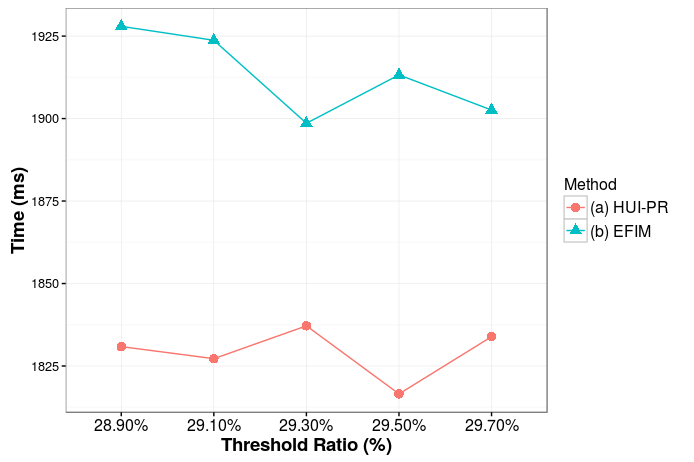
\includegraphics[scale=0.5]{RuntimeConnect-HUIPRvEFIM}
		\subcaption{Connect Dataset}
		\label{fig:graph-connect}
	\end{subfigure}    
	\begin{subfigure}{\textwidth}
		\centering
		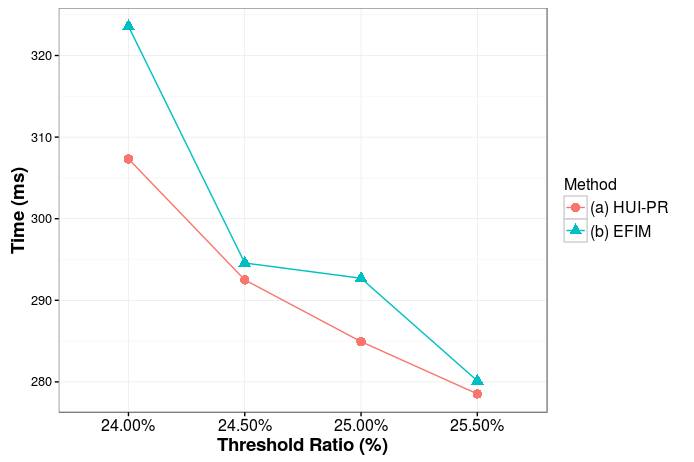
\includegraphics[scale=0.5]{RuntimeChess-HUIPRvEFIM}
		\subcaption{Chess Dataset}
		\label{fig:graph-chess}
	\end{subfigure}
	\begin{subfigure}{\textwidth}
		\centering 
		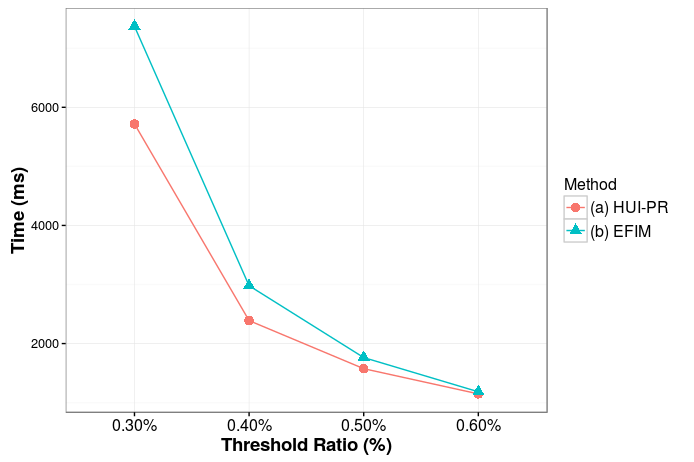
\includegraphics[scale=0.5]{RuntimeRetail-HUIPRvEFIM}
		\subcaption{Retail Dataset}
		\label{fig:graph-retail}
	\end{subfigure}
	\caption{Comparison of computational time between HUI-PR and EFIM w.r.t. variants of minimum threshold for different datasets}
	\label{fig:graph-comparison}
\end{figure}
\begin{figure}
	\centering 
	\begin{subfigure}[b]{\textwidth}
		\centering
		 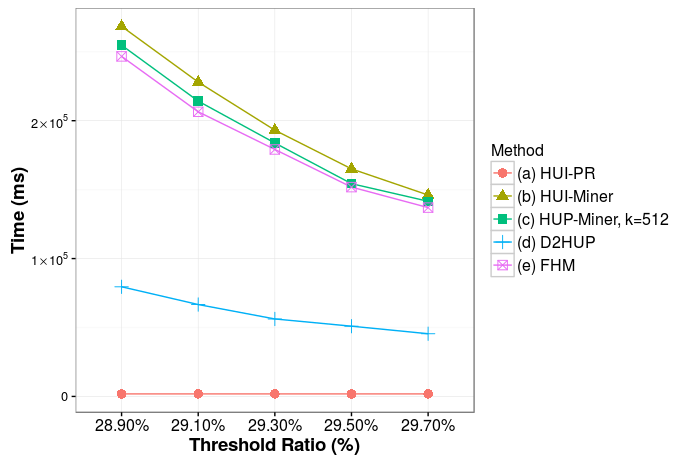
\includegraphics[scale=0.7]{RuntimeConnect-HUIPRvAll}
		\subcaption{Connect Dataset}
		\label{fig:graph-connect-comparison}
		\bigskip
	\end{subfigure}
	\begin{subfigure}[b]{\textwidth}
		\centering
		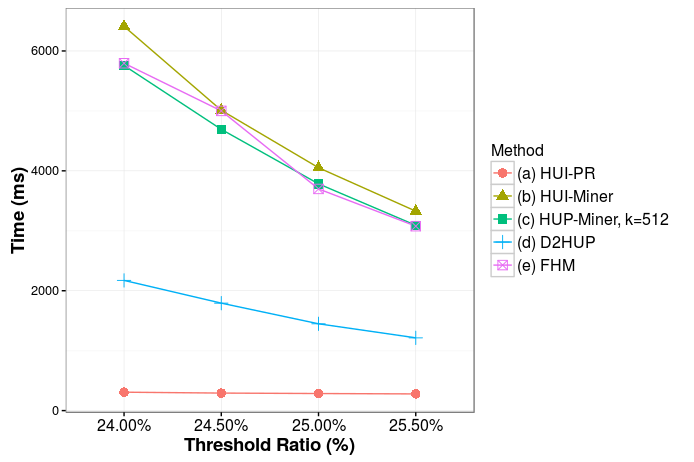
\includegraphics[scale=0.7]{RuntimeChess-HUIPRvAll}
		\subcaption{Chess Dataset}
		\label{fig:graph-chess-comparison}
	\end{subfigure}
	\caption{Comparison of computational time with state-of-the-art algorithms w.r.t. variants of minimum threshold}
	\label{fig:graph-multiple-comparison}
\end{figure}


\subsection{Comparison of HUIs}
From the experiments conducted on the real-world datasets (Connect, Chess and Retail), the number of HUIs found by both the experiments are same. We recorded the number of HUIs found for the range of threshold ratio for different datasets which are shown in Table \ref{table:result_huis}. For the ``Connect" database, we got 81 HUIs for 28.90\% and 4 HUIs for 29.70\%. Similarly, for the ``Chess" dataset, we got 342 HUIs for 24.00\% and 16 HUIs for 26.00\% threshold ratio. From the results obtained, we can verify that all the high utility itemsets have been found from our proposed algorithm HUI-PR.


\begin{table}
	\renewcommand{\arraystretch}{1.3}
	\caption{Total Number of HUIs found in HUI-PR and EFIM}
	\label{table:result_huis}
	\centering
	\begin{tabular}{|c||c|c|}
		\hline
		\bfseries Dataset & \bfseries ThresholdRatio $\delta$ & \bfseries \# of HUIs\\
		\hline\hline
		$Connect$ & 28.90\% & 81\\ \hline
		$Connect$ & 29.10\% & 40\\ \hline
		$Connect$ & 29.30\% & 20\\ \hline
		$Connect$ & 29.50\% & 8\\ \hline
		$Connect$ & 29.70\% & 4\\ \hline \hline
		
		$Chess$ & 24.00\% & 342\\ \hline
		$Chess$ & 24.50\% & 177\\ \hline
		$Chess$ & 25.00\% & 98\\ \hline
		$Chess$ & 25.50\% & 41\\ \hline
		$Chess$ & 26.00\% & 16\\ \hline \hline
		
		$Retail$ & 0.30\% & 92\\ \hline
		$Retail$ & 0.40\% & 58\\ \hline
		$Retail$ & 0.50\% & 41\\ \hline
		$Retail$ & 0.60\% & 30\\ \hline
		
	\end{tabular}
\end{table}

\begin{table}
	\renewcommand{\arraystretch}{1.3}
	\caption{Total Number of Transactions Pruned in HUI-PR}
	\label{result_transactions_pruned}
	\centering
	\begin{tabular}{|c||c|c|}
		\hline
		\bfseries Dataset & \bfseries ThresholdRatio $\delta$ & \bfseries \# Transactions Pruned\\        \hline\hline
		
		$Connect$ & 28.90\% & 556831\\ \hline
		$Connect$ & 29.10\% & 550630\\ \hline
		$Connect$ & 29.30\% & 550630\\ \hline
		$Connect$ & 29.50\% & 550630\\ \hline
		$Connect$ & 29.70\% & 550630\\ \hline \hline
		
		$Chess$ & 24.00\% & 24878\\ \hline
		$Chess$ & 24.50\% & 30779\\ \hline
		$Chess$ & 25.00\% & 27829\\ \hline
		$Chess$ & 25.50\% & 26265\\ \hline
		$Chess$ & 26.00\% & 26304\\ \hline \hline
		
		$Retail$ & 0.30\% & 670018\\ \hline
		$Retail$ & 0.40\% & 245342\\ \hline
		$Retail$ & 0.50\% & 117453\\ \hline
		$Retail$ & 0.60\% & 61939\\ \hline
		
	\end{tabular}
\end{table}


\subsection{Comparison of Candidate Sets}
From the Figure \ref{fig:comparison-candidatesets-efim}, we compared the candidate sets obtained from HUI-PR and EFIM algorithms. The candidate sets generated in HUI-PR are lower in number than that in EFIM algorithm. The candidate sets are minimized in the HUI-PR using transaction pruning strategies with pruning hash table and utility based pruning. For the ``Connect" dataset for threshold ratio 28.90\%, HUI-PR generated 3007 candidate sets while the EFIM algorithm generates 3132 candidate sets. HUI-PR could generate fewer candidate sets in the ``Chess" dataset. For 24.00\% threshold ratio, HUI-PR generated 2933 candidate itemsets while EFIM generated 2965 number of candidate itemsets. We also compared the candidate sets obtained from state-of-the-art algorithms: HUIMiner, FHM and FHM+ as shown in Figure \ref{fig:graph-candidatesets-comparison}. The number of candidate sets generated by our algorithm HUI-PR is 8 times less than HUIMiner and FHM for the ``Chess" dataset while HUI-PR generates 10 times less than HUIMiner and FHM for the ``Connect" dataset.

\begin{figure}
	\centering
	\begin{subfigure}[b]{\textwidth}
		\centering
		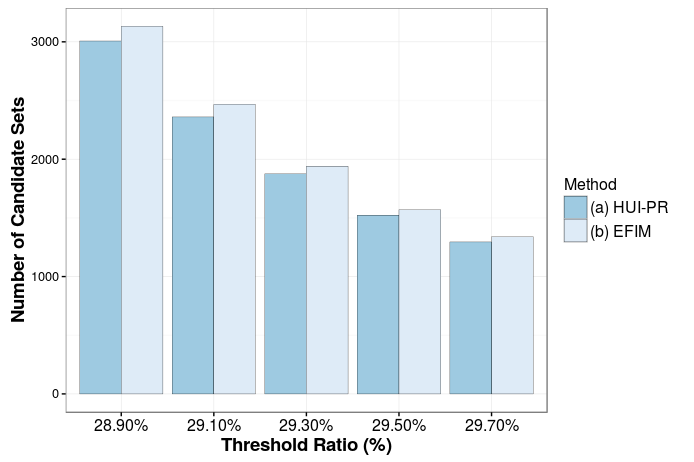
\includegraphics[scale=0.5]{CandidateSetsConnect-EFIM}
		\subcaption{Connect Dataset}\label{fig:connect-candidatesets}
	\end{subfigure}
	\begin{subfigure}[b]{\textwidth}
		\centering
		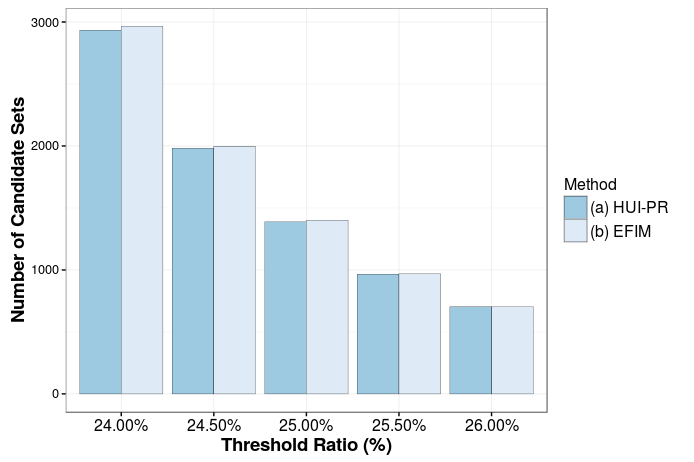
\includegraphics[scale=0.5]{CandidateSetsChess-EFIM}
		\subcaption{Chess Dataset}\label{fig:chess-candidatesets}
	\end{subfigure}
	\begin{subfigure}[b]{\textwidth}
		\centering
		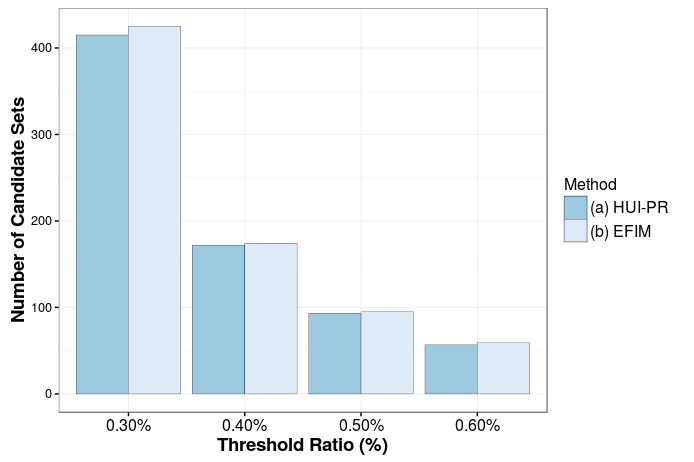
\includegraphics[scale=0.5]{CandidateSetsRetail-EFIM}
		\subcaption{Retail Dataset}\label{fig:retail-candidatesets}
	\end{subfigure}
	\caption{Comparison of candidate sets between HUI-PR and EFIM w.r.t. variants of minimum threshold}
	\label{fig:comparison-candidatesets-efim}
\end{figure}

\begin{figure}
	\centering
	\begin{subfigure}[b]{\textwidth}
		\centering
		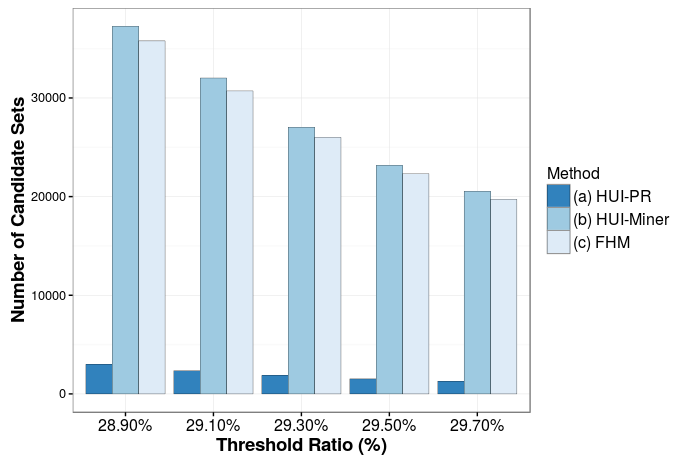
\includegraphics[scale=0.7]{CandidateSetsConnect-HUIPRvsAll}
		\subcaption{Connect Dataset}
		\label{fig:graph-connect-candidatesets}
		\bigskip
	\end{subfigure}
	\begin{subfigure}[b]{\textwidth}
		\centering
		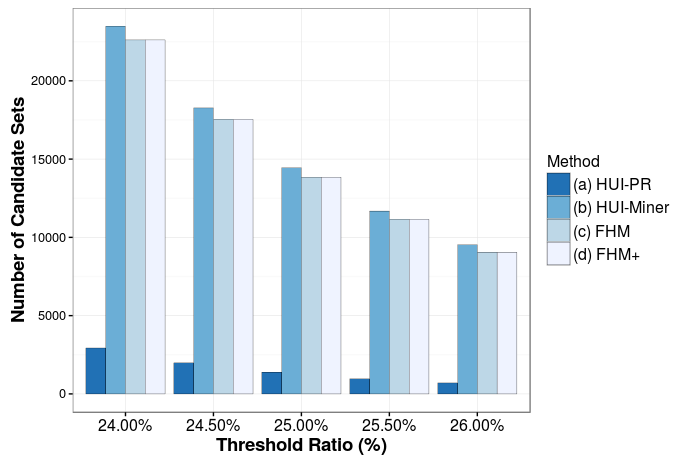
\includegraphics[scale=0.7]{CandidateSetsChess-HUIPRvsAll}
		\subcaption{Chess Dataset}\label{fig:graph-chess-candidatesets}
	\end{subfigure}
	\caption{Comparison of candidate sets with state-of-the-art algorithms w.r.t. variants of minimum threshold}
	\label{fig:graph-candidatesets-comparison}
\end{figure}

\section{EFIM-Par vs EFIM}
We compared our proposed distributed algorithm Parallel EFIM (EFIM-Par) with Approximate parallel high utility itemset mining (PHUI-Miner) \cite{Chen2016}. The computational time were recorded for the different datasets as shown in the Figure \ref{fig:graph-comparison-distributed}. These algorithms were performed on the larger datasets. Our algorithm were conducted on one master node and ten slave nodes in the Spark Framework.

\subsection{Comparison of Computational Time}
In this section, we ran our experiments on the real-world datasets (Connect, Chess, BMS and Mushroom). However, in order to make the datasets sufficiently large, we multiplied the ``Connect" dataset by a factor of 2, ``Chess" dataset by a factor of 30, ``BMS" dataset by a factor of 4 and ``Mushroom" dataset by a factor of 20. The experiments were conducted on our proposed algorithm EFIM-Par and PHUI-Miner.

From the Figure \ref{fig:graph-connect2x-distributed}, our algorithm EFIM-Par took 76.36 seconds while PHUI-Miner took 161.76 seconds for the threshold ratio 28.90\% for the ``Connect" dataset. Similarly, for the threshold ratio 29.70\%, our EFIM-Par took 64.42 seconds while PHUI-Miner took 113.27 seconds. Our algorithm EFIM-Par was able to perform around 2 times better than PHUI-Miner for the ``Connect" dataset for different threshold ratio taken. From the Figure \ref{fig:graph-chess30x-distributed}, for the ``Chess30x" dataset, our algorithm took 60.77 seconds for the threshold ratio 24.00\% while PHUI-Miner took 79.19 seconds. Similarly, for the threshold ratio 26.00\%, EFIM-Par took 51.97 seconds while PHUI-Miner took 71.03 seconds. Our algorithm performed almost 1.5 times better than PHUI-Miner for the ``Chess30x" dataset. Similarly for the ``BMS4x" dataset, our algorithm performed better for the lower threshold and almost similar for the higher threshold values. Our algorithm performed better than 1.2 times the PHUI-Miner algorithm for ``Mushroom20x" dataset.

\subsection{Comparison of HUIs}
From the Table \ref{table:result-huis-distributed}, we found that our algorithm EFIM-Par found the same number of HUIs as found by PHUI-Miner. Therefore, we can conclude our algorithm is as accurate as PHUI-Miner.

\begin{figure}
	%    \centering
	\begin{subfigure}{\textwidth}
		\centering
		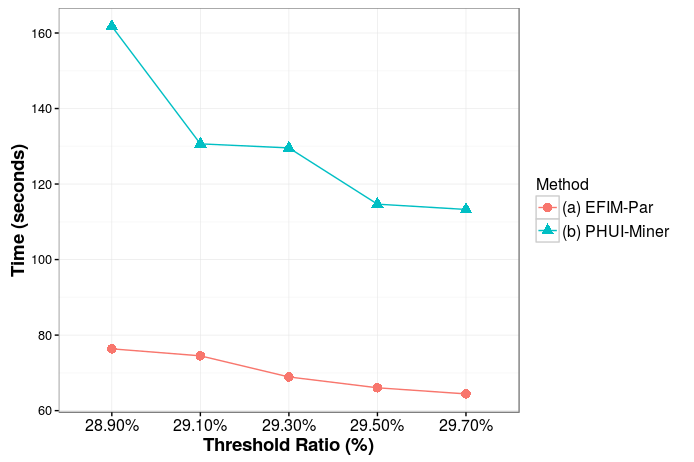
\includegraphics[scale=0.6]{RuntimeConnect2x-Distributed}
		\subcaption{Connect2x Dataset}
		\label{fig:graph-connect2x-distributed} 
		\bigskip
	\end{subfigure}    
	\begin{subfigure}{\textwidth}
		\centering
		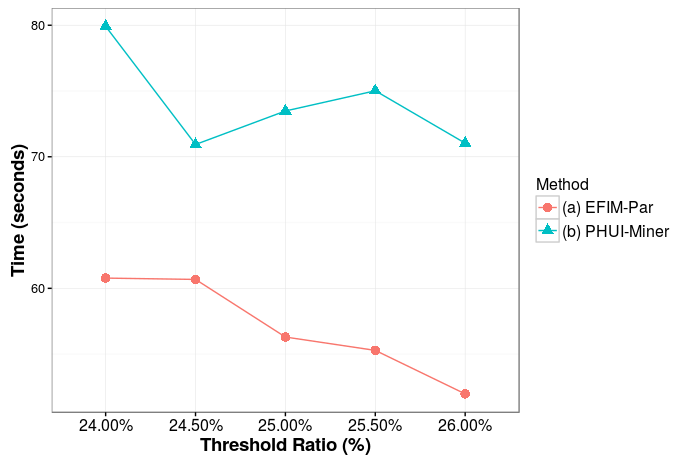
\includegraphics[scale=0.6]{RuntimeChess30x-Distributed}
		\subcaption{Chess30x Dataset}
		\label{fig:graph-chess30x-distributed}
	\end{subfigure}
	\caption{Comparison of computational time between EFIM-Par and PHUI-Miner w.r.t. variants of minimum threshold for different datasets}
\end{figure}
\begin{figure} \ContinuedFloat
	\begin{subfigure}{\textwidth}
		\centering
		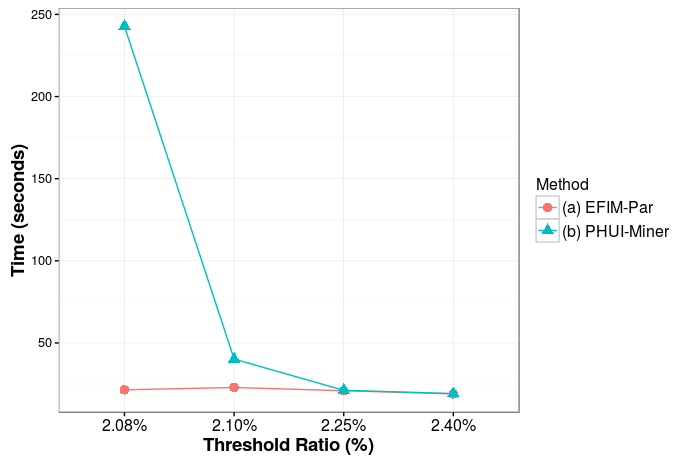
\includegraphics[scale=0.6]{RuntimeBMS4x-Distributed}
		\subcaption{BMS4x Dataset}
		\label{fig:graph-bms-distributed} 
		\bigskip
	\end{subfigure}
	\begin{subfigure}{\textwidth}
		\centering
		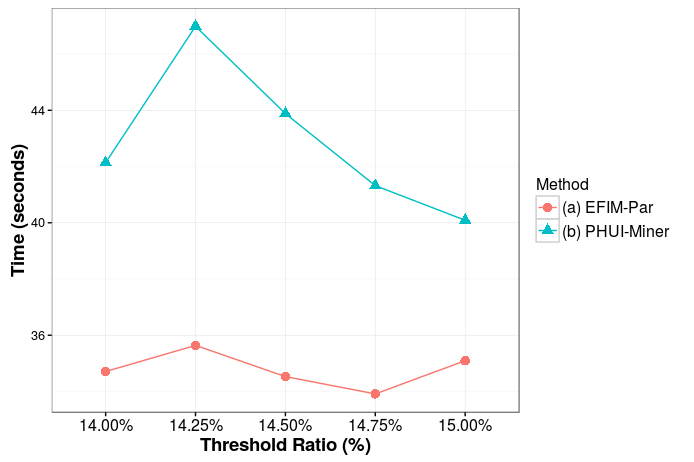
\includegraphics[scale=0.6]{RuntimeMushroom20x-Distributed}
		\subcaption{Mushroom20x Dataset}
		\label{fig:graph-mushroom20x-distributed} 
	\end{subfigure}
	\caption{Comparison of computational time between EFIM-Par and PHUI-Miner w.r.t. variants of minimum threshold for different datasets}
	\label{fig:graph-comparison-distributed}
\end{figure}

\begin{table}
	\renewcommand{\arraystretch}{1.3}
	\caption{Total Number of HUIs found in EFIM-Par and PHUI-Miner}
	\label{table:result-huis-distributed}
	\centering
	\begin{tabular}{|c||c|c|}
		\hline
		\bfseries Dataset & \bfseries ThresholdRatio $\delta$ & \bfseries \# of HUIs\\
		\hline\hline
		$Connect2x$ & 28.90\% & 81\\ \hline
		$Connect2x$ & 29.10\% & 40\\ \hline
		$Connect2x$ & 29.30\% & 20\\ \hline
		$Connect2x$ & 29.50\% & 8\\ \hline
		$Connect2x$ & 29.70\% & 4\\ \hline \hline
		
		$Chess30x$ & 24.00\% & 342\\ \hline
		$Chess30x$ & 24.50\% & 177\\ \hline
		$Chess30x$ & 25.00\% & 98\\ \hline
		$Chess30x$ & 25.50\% & 41\\ \hline
		$Chess30x$ & 26.00\% & 16\\ \hline \hline
		
		$BMS$ & 2.08\% & 7\\ \hline
		$BMS$ & 2.10\% & 7\\ \hline
		$BMS$ & 2.40\% & 5\\ \hline
		$BMS$ & 2.80\% & 3\\ \hline
		$BMS$ & 3.00\% & 2\\ \hline
		
		$Mushroom20x$ & 14.00\% & 67\\ \hline
		$Mushroom20x$ & 14.25\% & 38\\ \hline
		$Mushroom20x$ & 14.50\% & 19\\ \hline
		$Mushroom20x$ & 14.75\% & 10\\ \hline
		$Mushroom20x$ & 15.00\% & 2\\ \hline
		
	\end{tabular}
\end{table}


\chapter{Conclusion and Future Work} \label{chapter:conclusion}
In this thesis, two methods HUI-PR and EFIM-Par have been proposed. The proposed algorithm (HUI-PR) is a novel approach of pruning transactions to reduce the search space while finding high utility itemsets. HUI-PR can reduce the search space by eliminating the number of candidate sets which avoids the computation of unnecessary itemsets. HUI-PR uses a pruning hash table, which stores low-utility itemsets that are checked while generating the projected transaction in each node. This elimination helps reduce the candidate sets in HUI-PR besides different utilities such as sub-tree utility, local utility and transaction weighted utility for pruning. This approach is highly suited for comparatively smaller datasets. Another proposed algorithm (EFIM-Par) is a novel approach to mine high utility itemsets using distributed approach. Spark framework is used for the distributed computing because of its advantage over the Hadoop framework. Spark framework uses in-memory computation which is much faster than disk dependent Hadoop framework. Our algorithm divides the computation into multiple stages such that each task is divided into multiple worker nodes. In the mining stage, each work gets the task using the grouping mechanism which finds the high utility itemsets that are aggregated to find the overall high utility itemsets. An extensive experiment in various datasets with the state-of-the-art algorithm is conducted for both methods. Our experiments show that HUI-PR can perform more efficiently than other existing algorithms. HUI-PR improves the computational time for finding the high utility itemsets as it reduces the number of candidate sets. HUI-PR gains significant performance improvement in terms of computational time and a number of candidates sets generated. Our experiments for EFIM-Par shows that it performs better than PHUI-Miner. Our algorithm performs much better in terms of computation than PHUI-Miner. EFIM-Par divides the search space in an efficient way so that each worker nodes compute in faster time.

Although our proposed methods perform much better than other algorithms, these methods could be enhanced to perform at optimum level. Our algorithm (HUI-PR) finds the high utility itemsets efficiently for small datasets. However, it has lessened improvement when the datasets are very small. Therefore, an improvement could be done for very small datasets. Also, different tree construction mechanisms could be studied so that the proposed pruning strategies can work best. Our other algorithm (EFIM-Par) could be enhanced with much better grouping mechanism to divide the tasks to each worker node in an optimum manner.



%%%
%%% The bibliography - you can change the alpha to suit your style if you don't like it is it is.
%%% The bib file should be called 'thesis.bib' - if not then change the second line here to be correct.
\bibliographystyle{alpha}
\thesisbibliography{thesis}


%%%
%%% Vita comes next
\vita
\chapter{} %% please leave this one blank - the vita stuff is sort of a hack.
\linespread{1.3} 
\begin{center}
Graduate College\\
University of Nevada, Las Vegas\\[1cm]
Aditya Rajuladevi\\[1cm]
\end{center}

\noindent Degrees:\\
\indent Bachelor Degree in Computer Engineering 2014\\
\indent Jawaharlal Nehru Technological University, Hyderabad, India\\

\noindent Thesis Title: A Machine Learning Approach to Predict First-Year Student Retention Rates at University of Nevada, Las Vegas\\

\noindent Thesis Examination Committee:\\
\indent Chairperson, Dr. Fatma Nasoz, Ph.D.\\
\indent Committee Member, Dr. Laxmi Gewali, Ph.D.\\
\indent Committee Member, Dr. Justin Zhan, Ph.D.\\
\indent Graduate Faculty Representative, Dr. Magdalena Martinez, Ph.D.\\

\end{document}





